如果想要直接使用程序, 只需要使用cmake编译后运行./main, 即可看到帮助信息,
并据此使用程序.\par

对程序的测试使用GoogleTest,
下面将通过先整体展示后对具体模块逐个展示的方式进行展示. 具体内容如下:
\subsection{LL(1)语法分析程序}
\subsubsection{整体测试}
使用简单的文法和作业所给文法进行测试, 使用的简单文法和复杂文法如下:
\lstinputlisting[language=c++]{../grammars/g1.txt}
\lstinputlisting[language=c++]{../grammars/g2.txt}
对简单文法, 得到first集和follow集, 语法分析表如图\ref{fig:简单文法的语法分析表}.
\begin{figure}[ht!]
	\begin{center}
		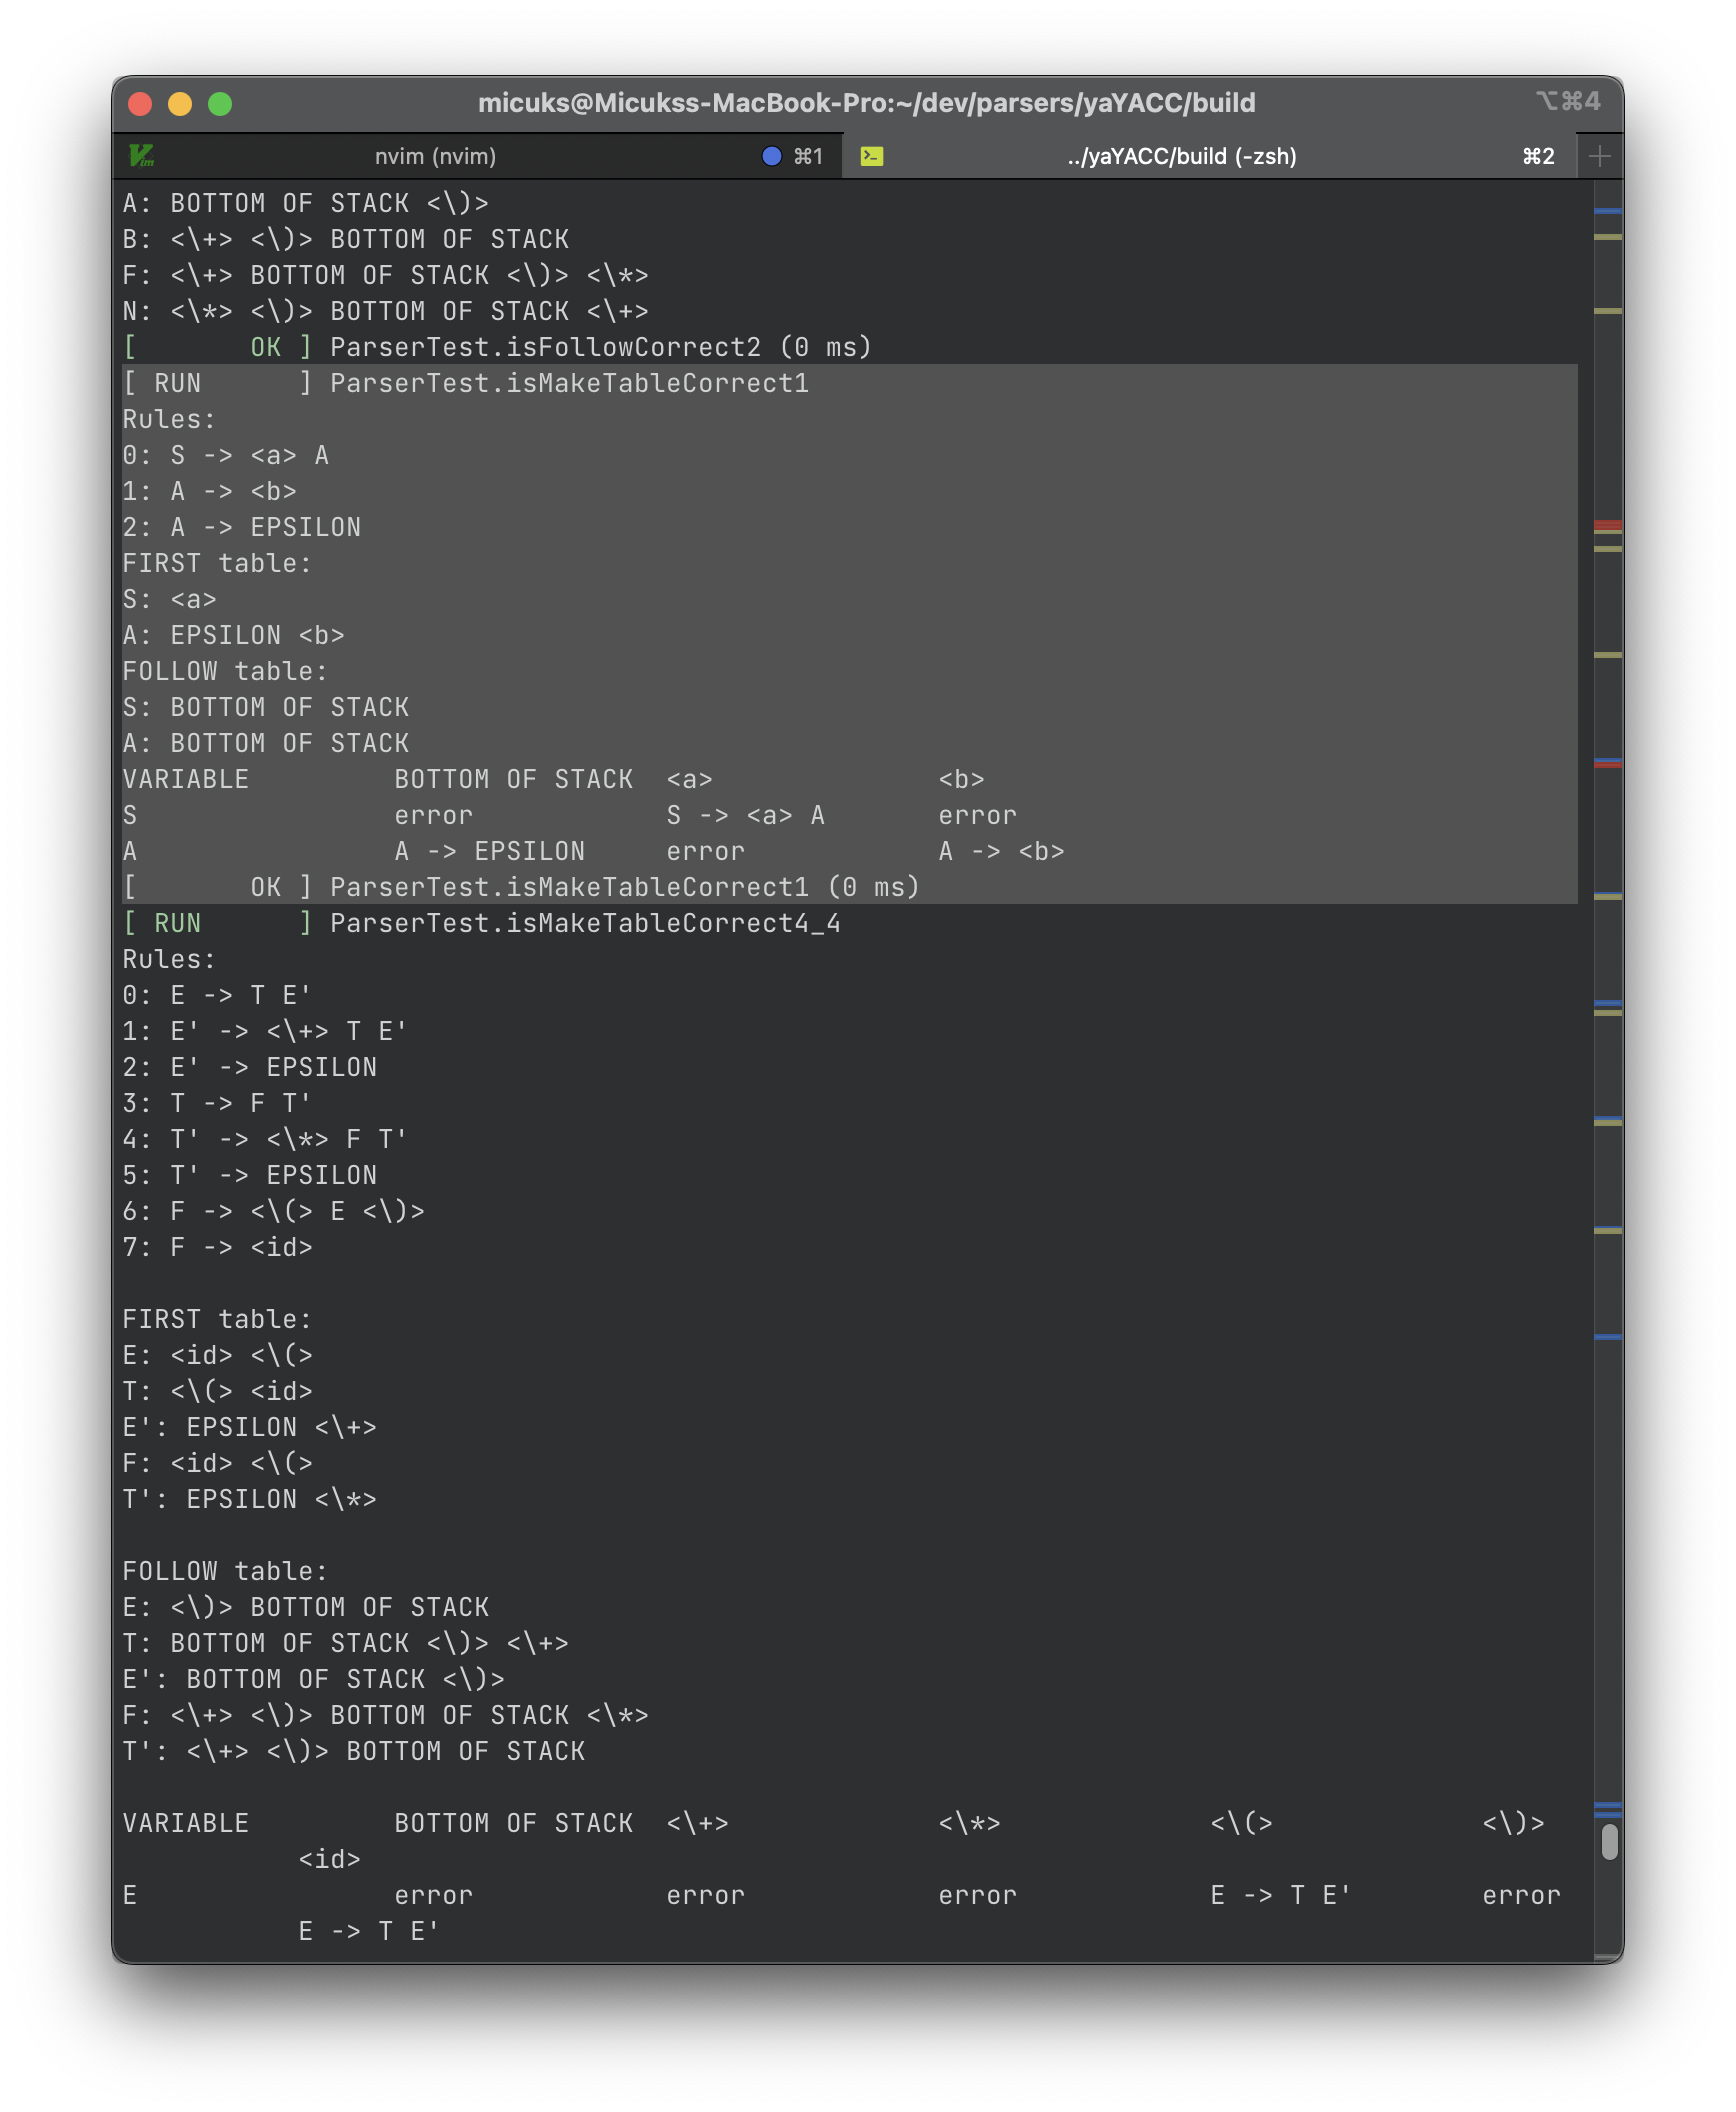
\includegraphics[width=0.95\textwidth]{figures/ll1分析表1.png}
	\end{center}
	\caption{简单文法的语法分析表}
	\label{fig:简单文法的语法分析表}
\end{figure}

较复杂的文法进行测试, 同样得到正确输出, 如图\ref{fig:复杂文法的语法分析表}.
\lstinputlisting[language=c++]{../grammars/g2.txt}

\begin{figure}[ht!]
	\begin{center}
		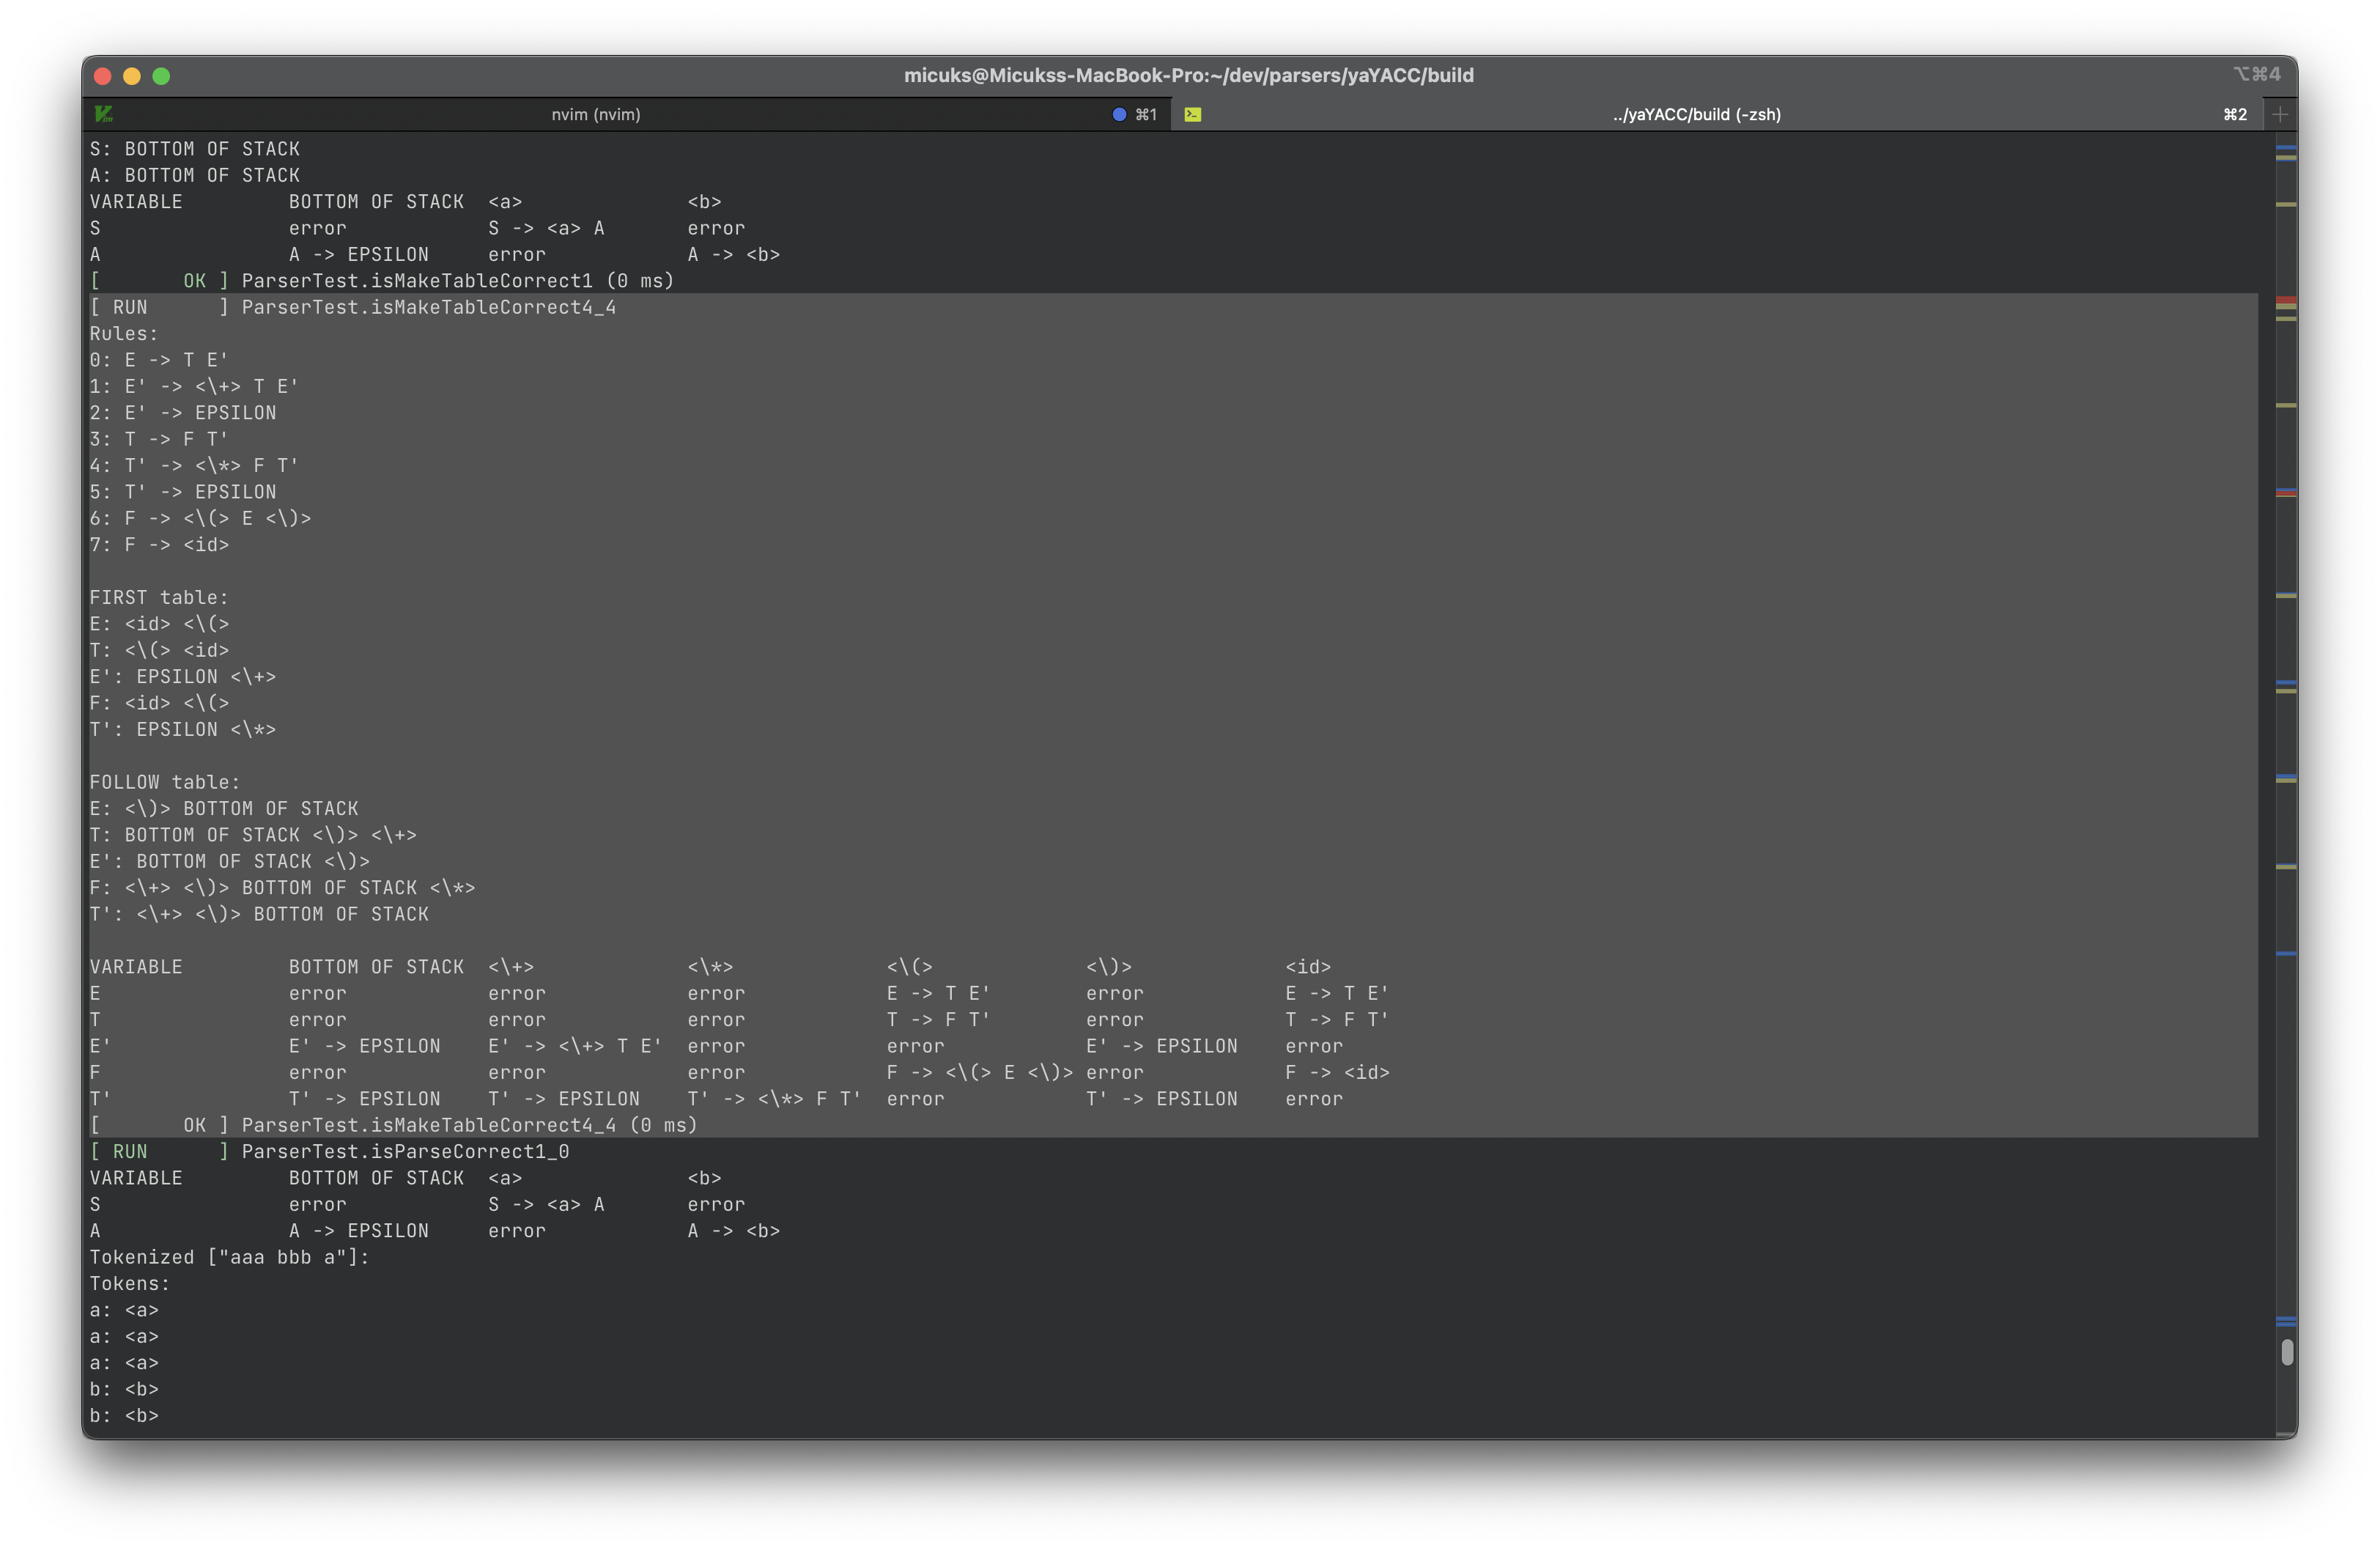
\includegraphics[width=0.95\textwidth]{figures/ll1分析表2.png}
	\end{center}
	\caption{复杂文法的语法分析表}
	\label{fig:复杂文法的语法分析表}
\end{figure}

使用简单文法生成的LL(1)分析表对字符串进行分析如图\ref{fig:简单文法的语法分析}. 两个字符串分别为"aaa bbb a", 和"   a
b   ", 其中, 第一个字符串会被拒绝, 第二个字符串会被接受,
关于程序结果是否正确的判断, 都是写在googletest中的检测内容, 具体可以见文末的代码清单.

\begin{figure}[ht!]
	\begin{center}
		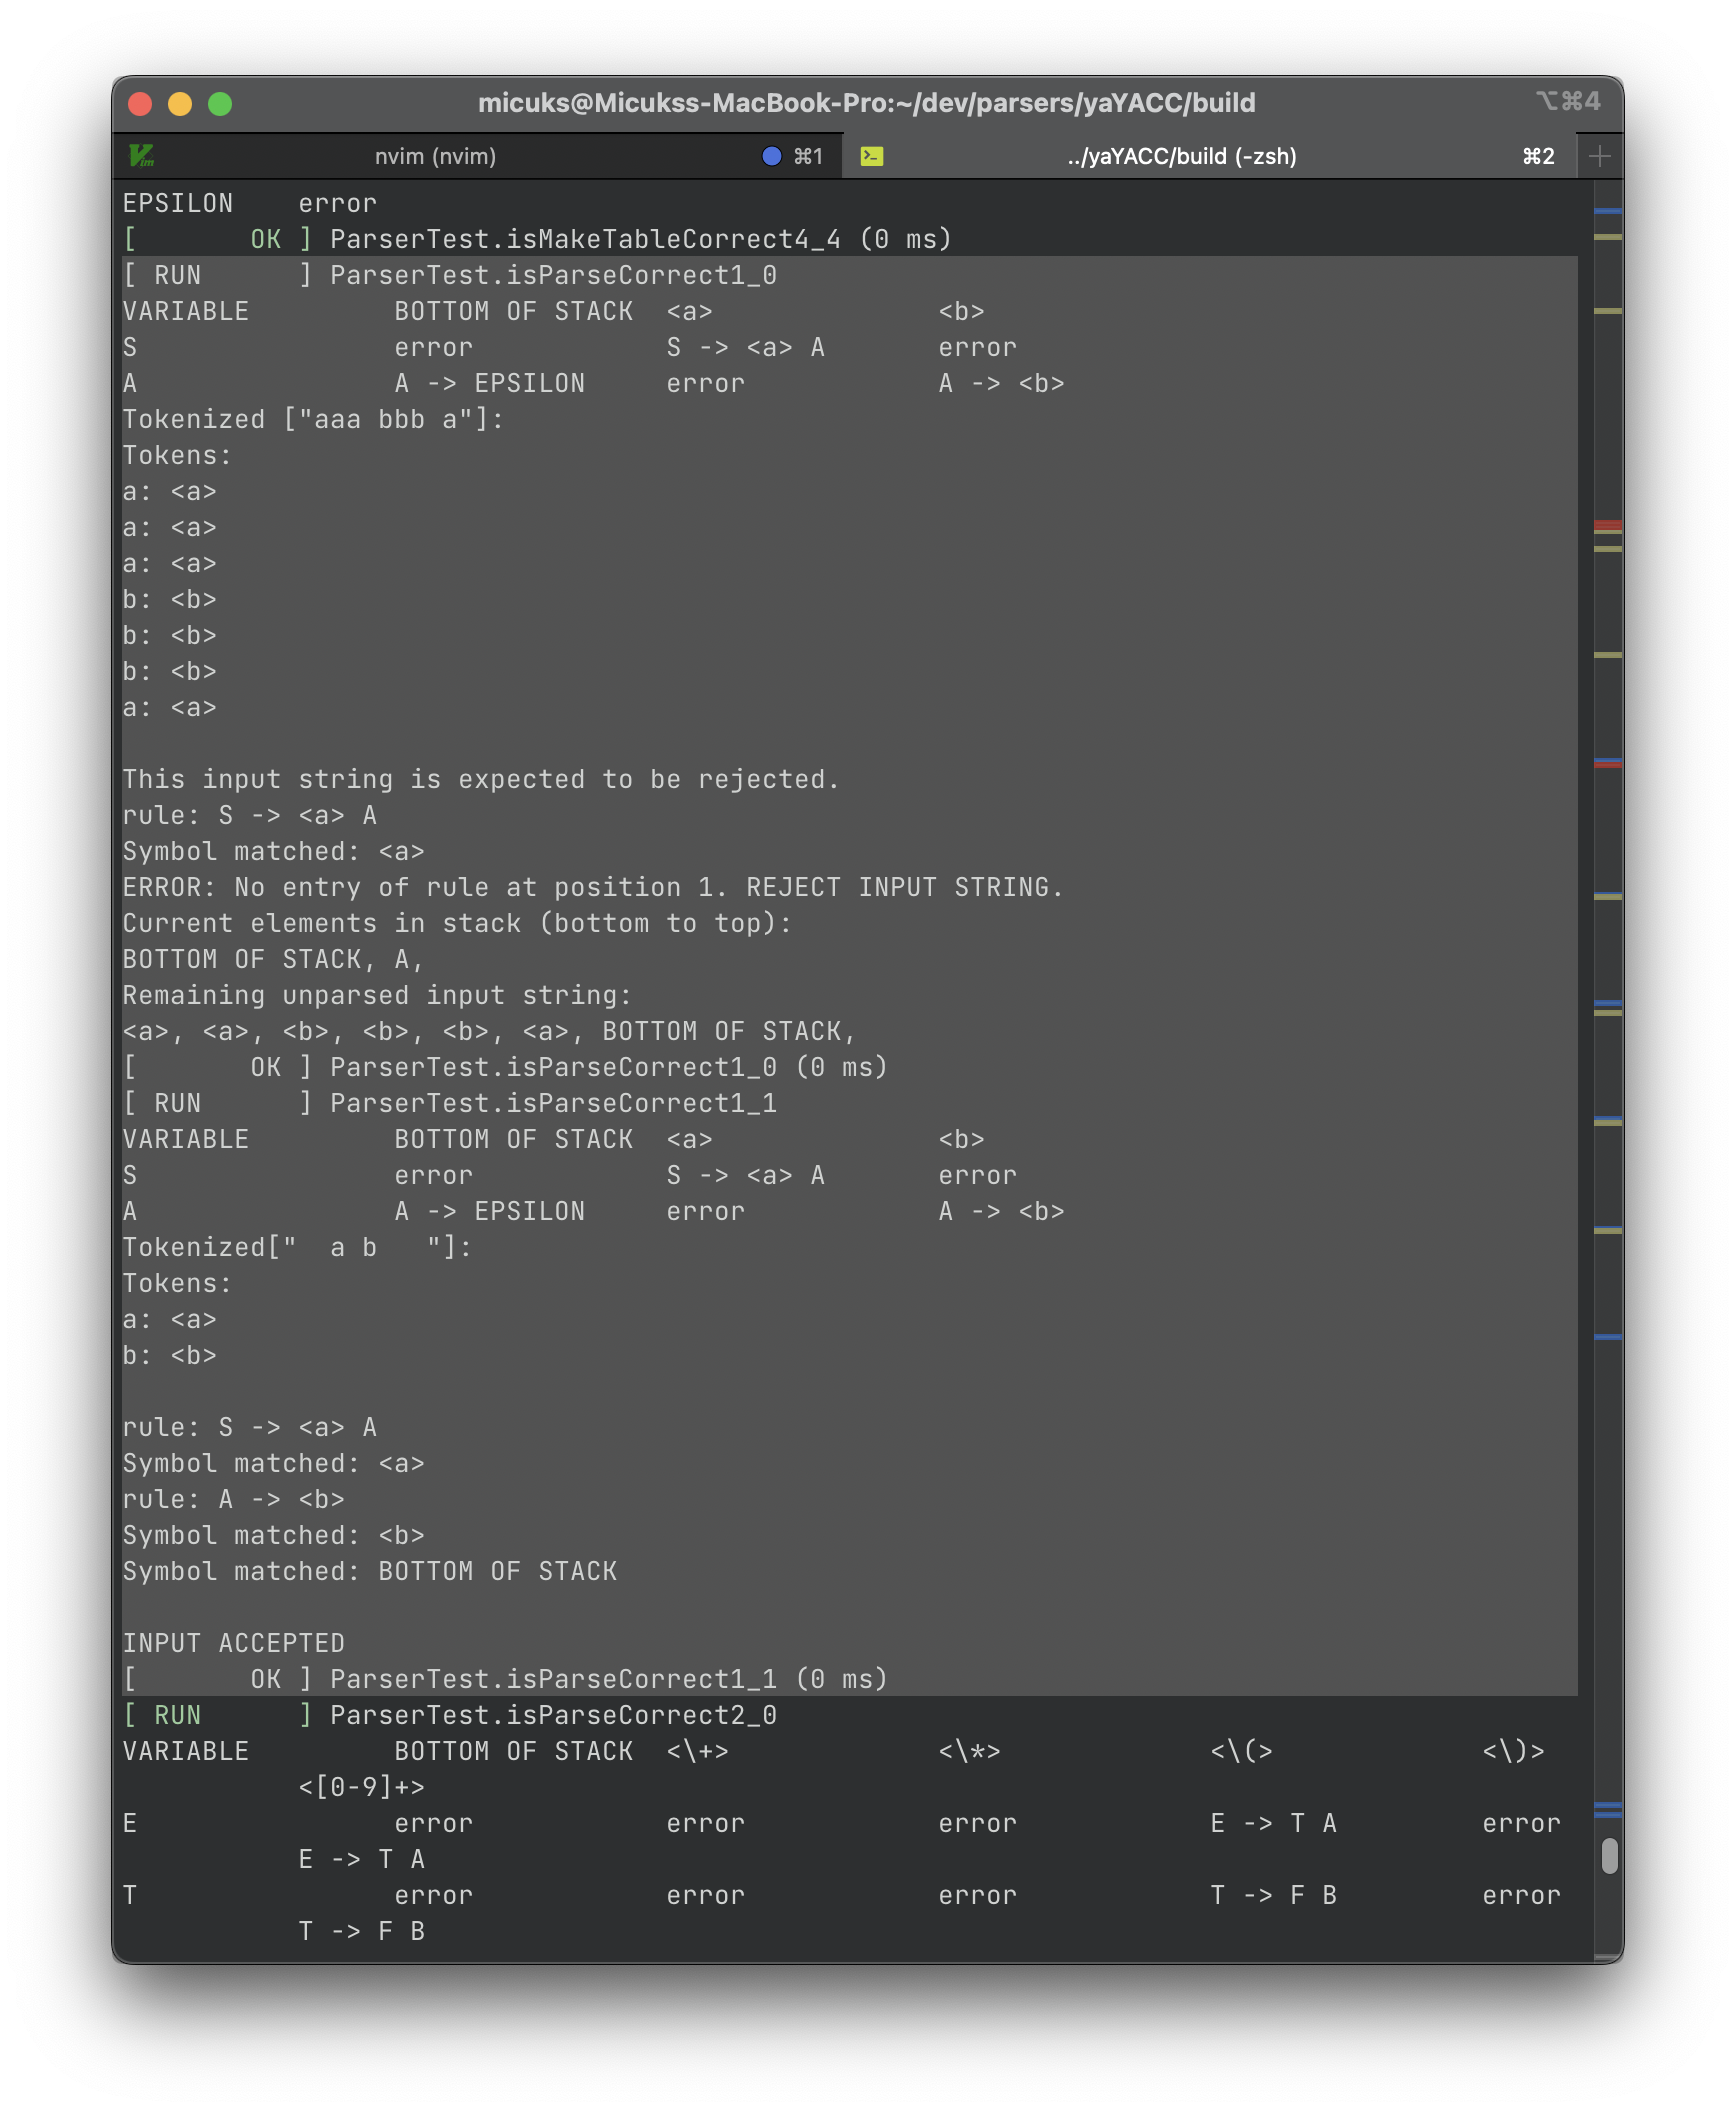
\includegraphics[width=0.95\textwidth]{figures/ll1分析输入1.png}
	\end{center}
	\caption{简单文法的语法分析}
	\label{fig:简单文法的语法分析}
\end{figure}

使用复杂文法进行分析同样得到正确结果, 如图\ref{fig:复杂文法的语法分析}.
输入串为"1+2+3+", 会被拒绝.

\begin{figure}[ht!]
	\begin{center}
		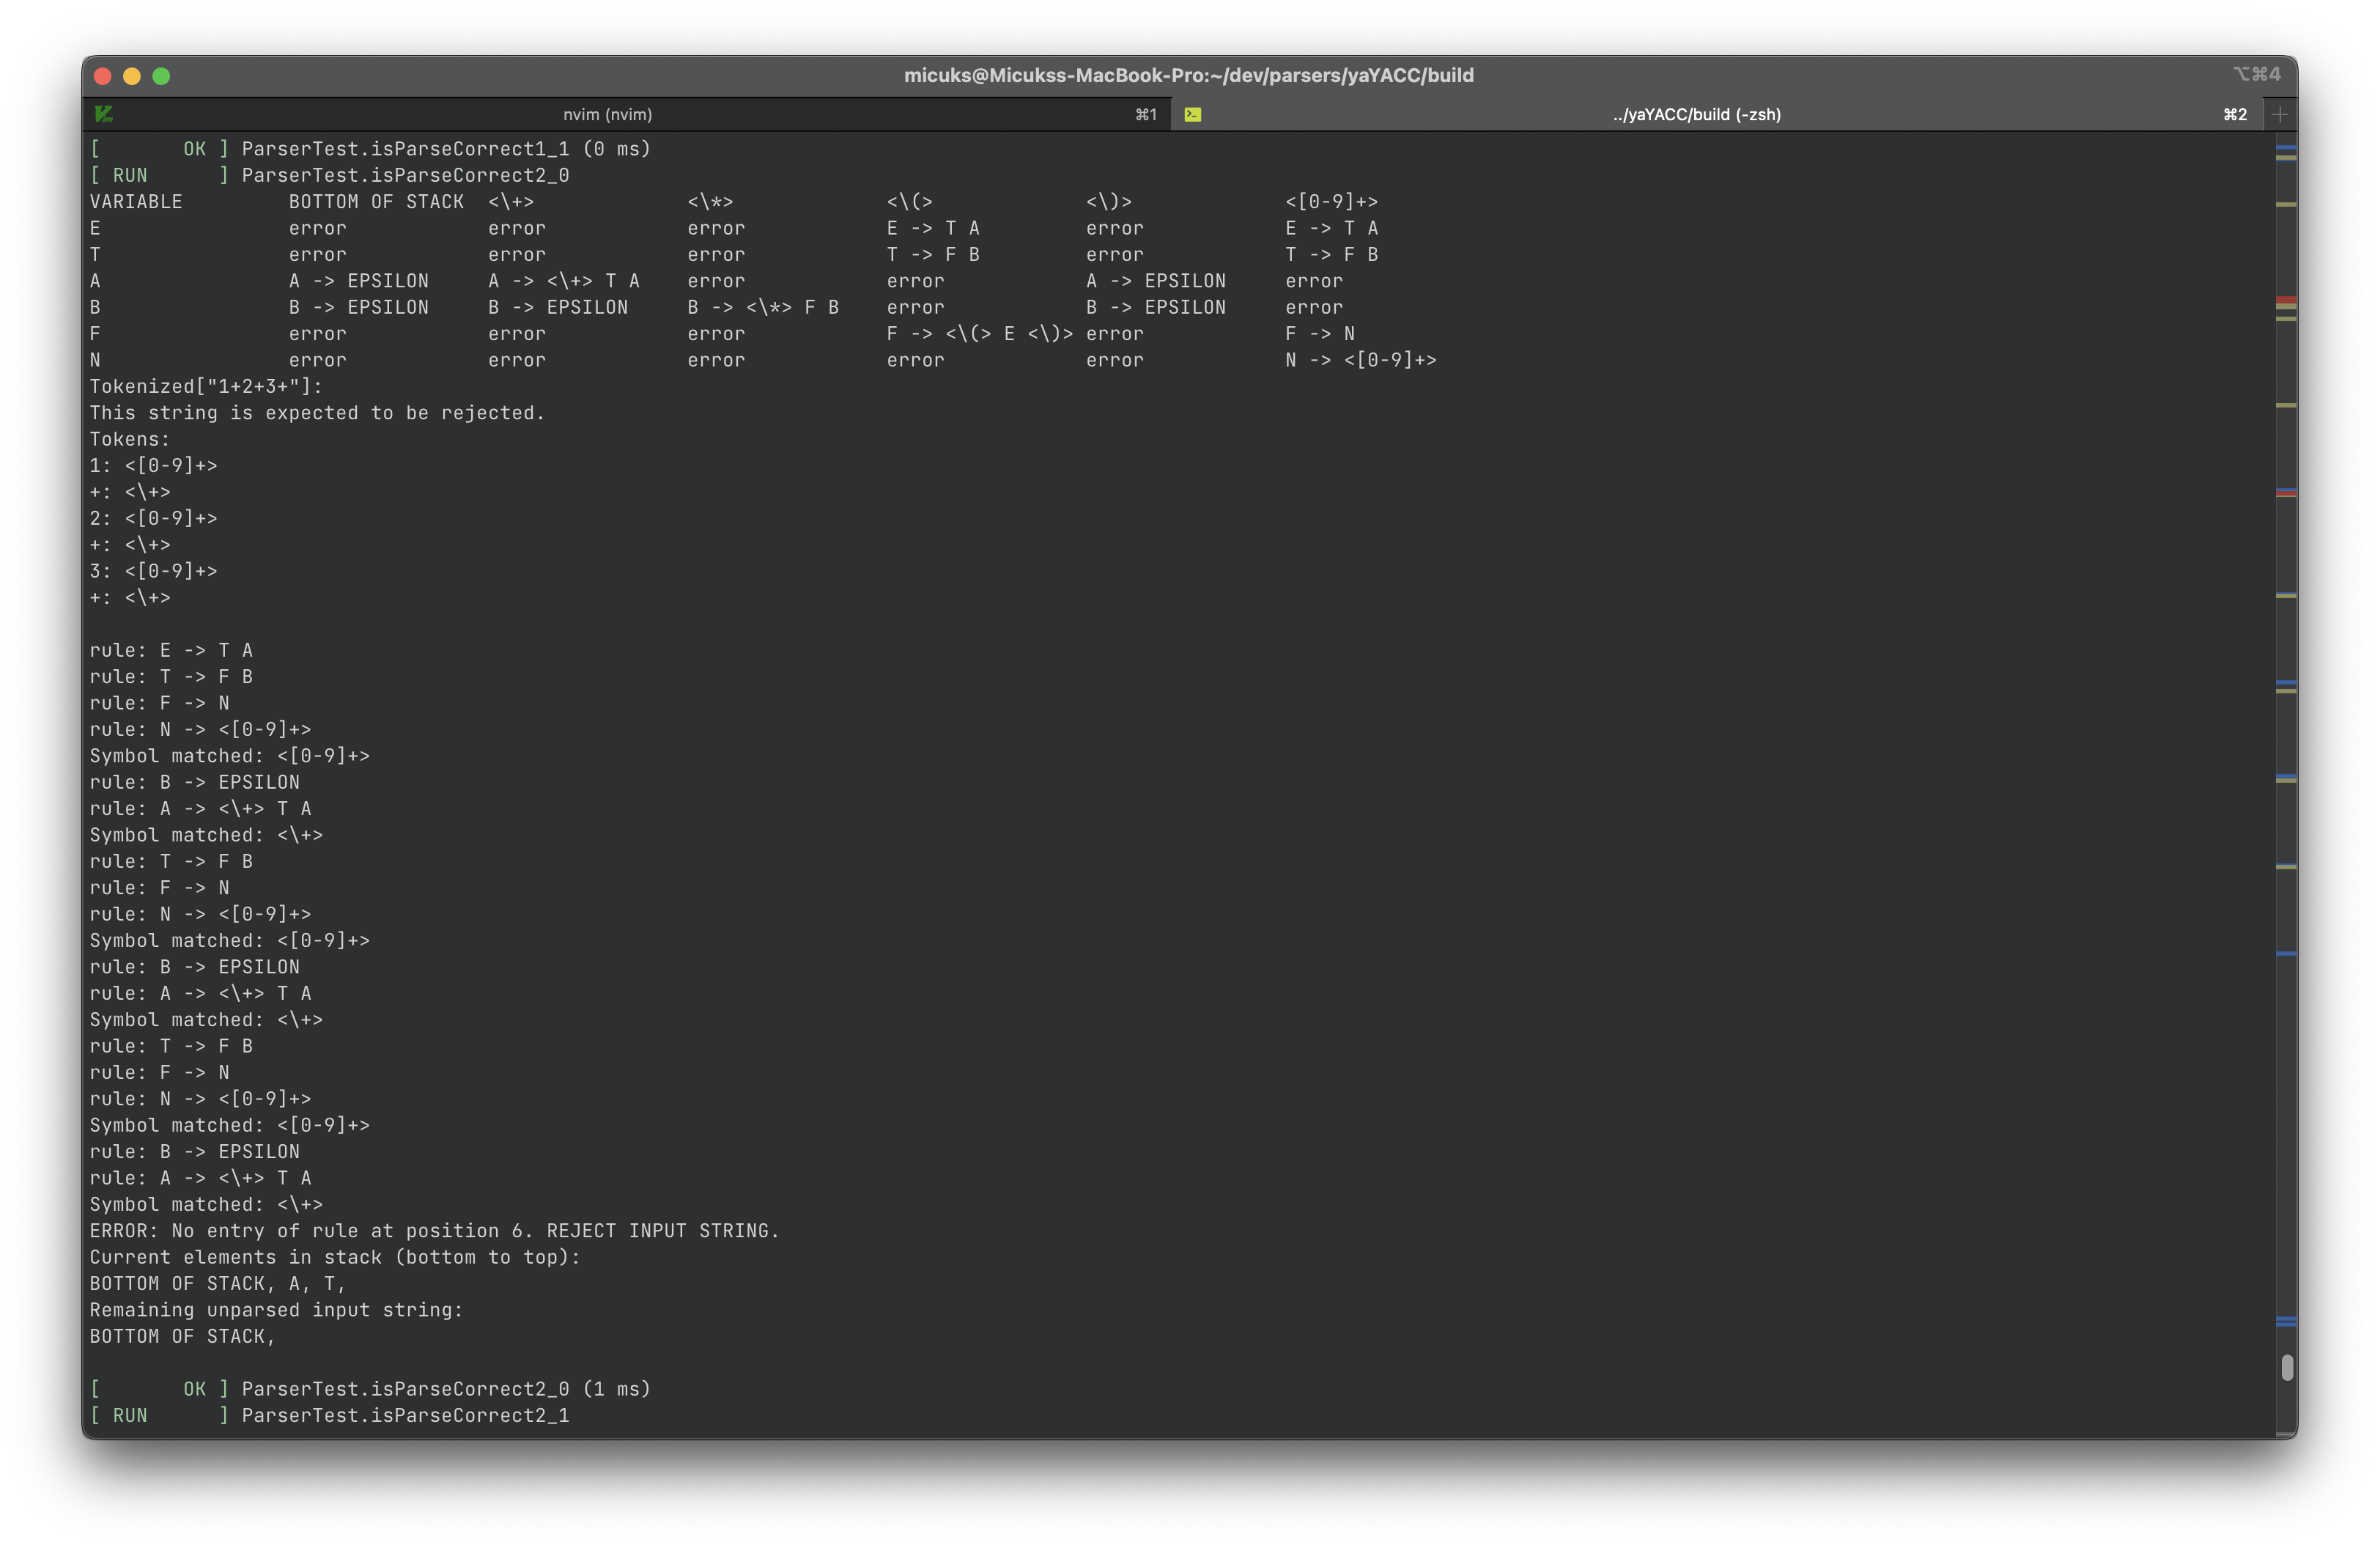
\includegraphics[width=0.95\textwidth]{figures/ll1分析输入20.png}
	\end{center}
	\caption{复杂文法的语法分析}
	\label{fig:复杂文法的语法分析}
\end{figure}

分析另一字符串"423*384*23", 将被接受, 如图\ref{fig:复杂文法的语法分析2}.

\begin{figure}[ht!]
	\begin{center}
		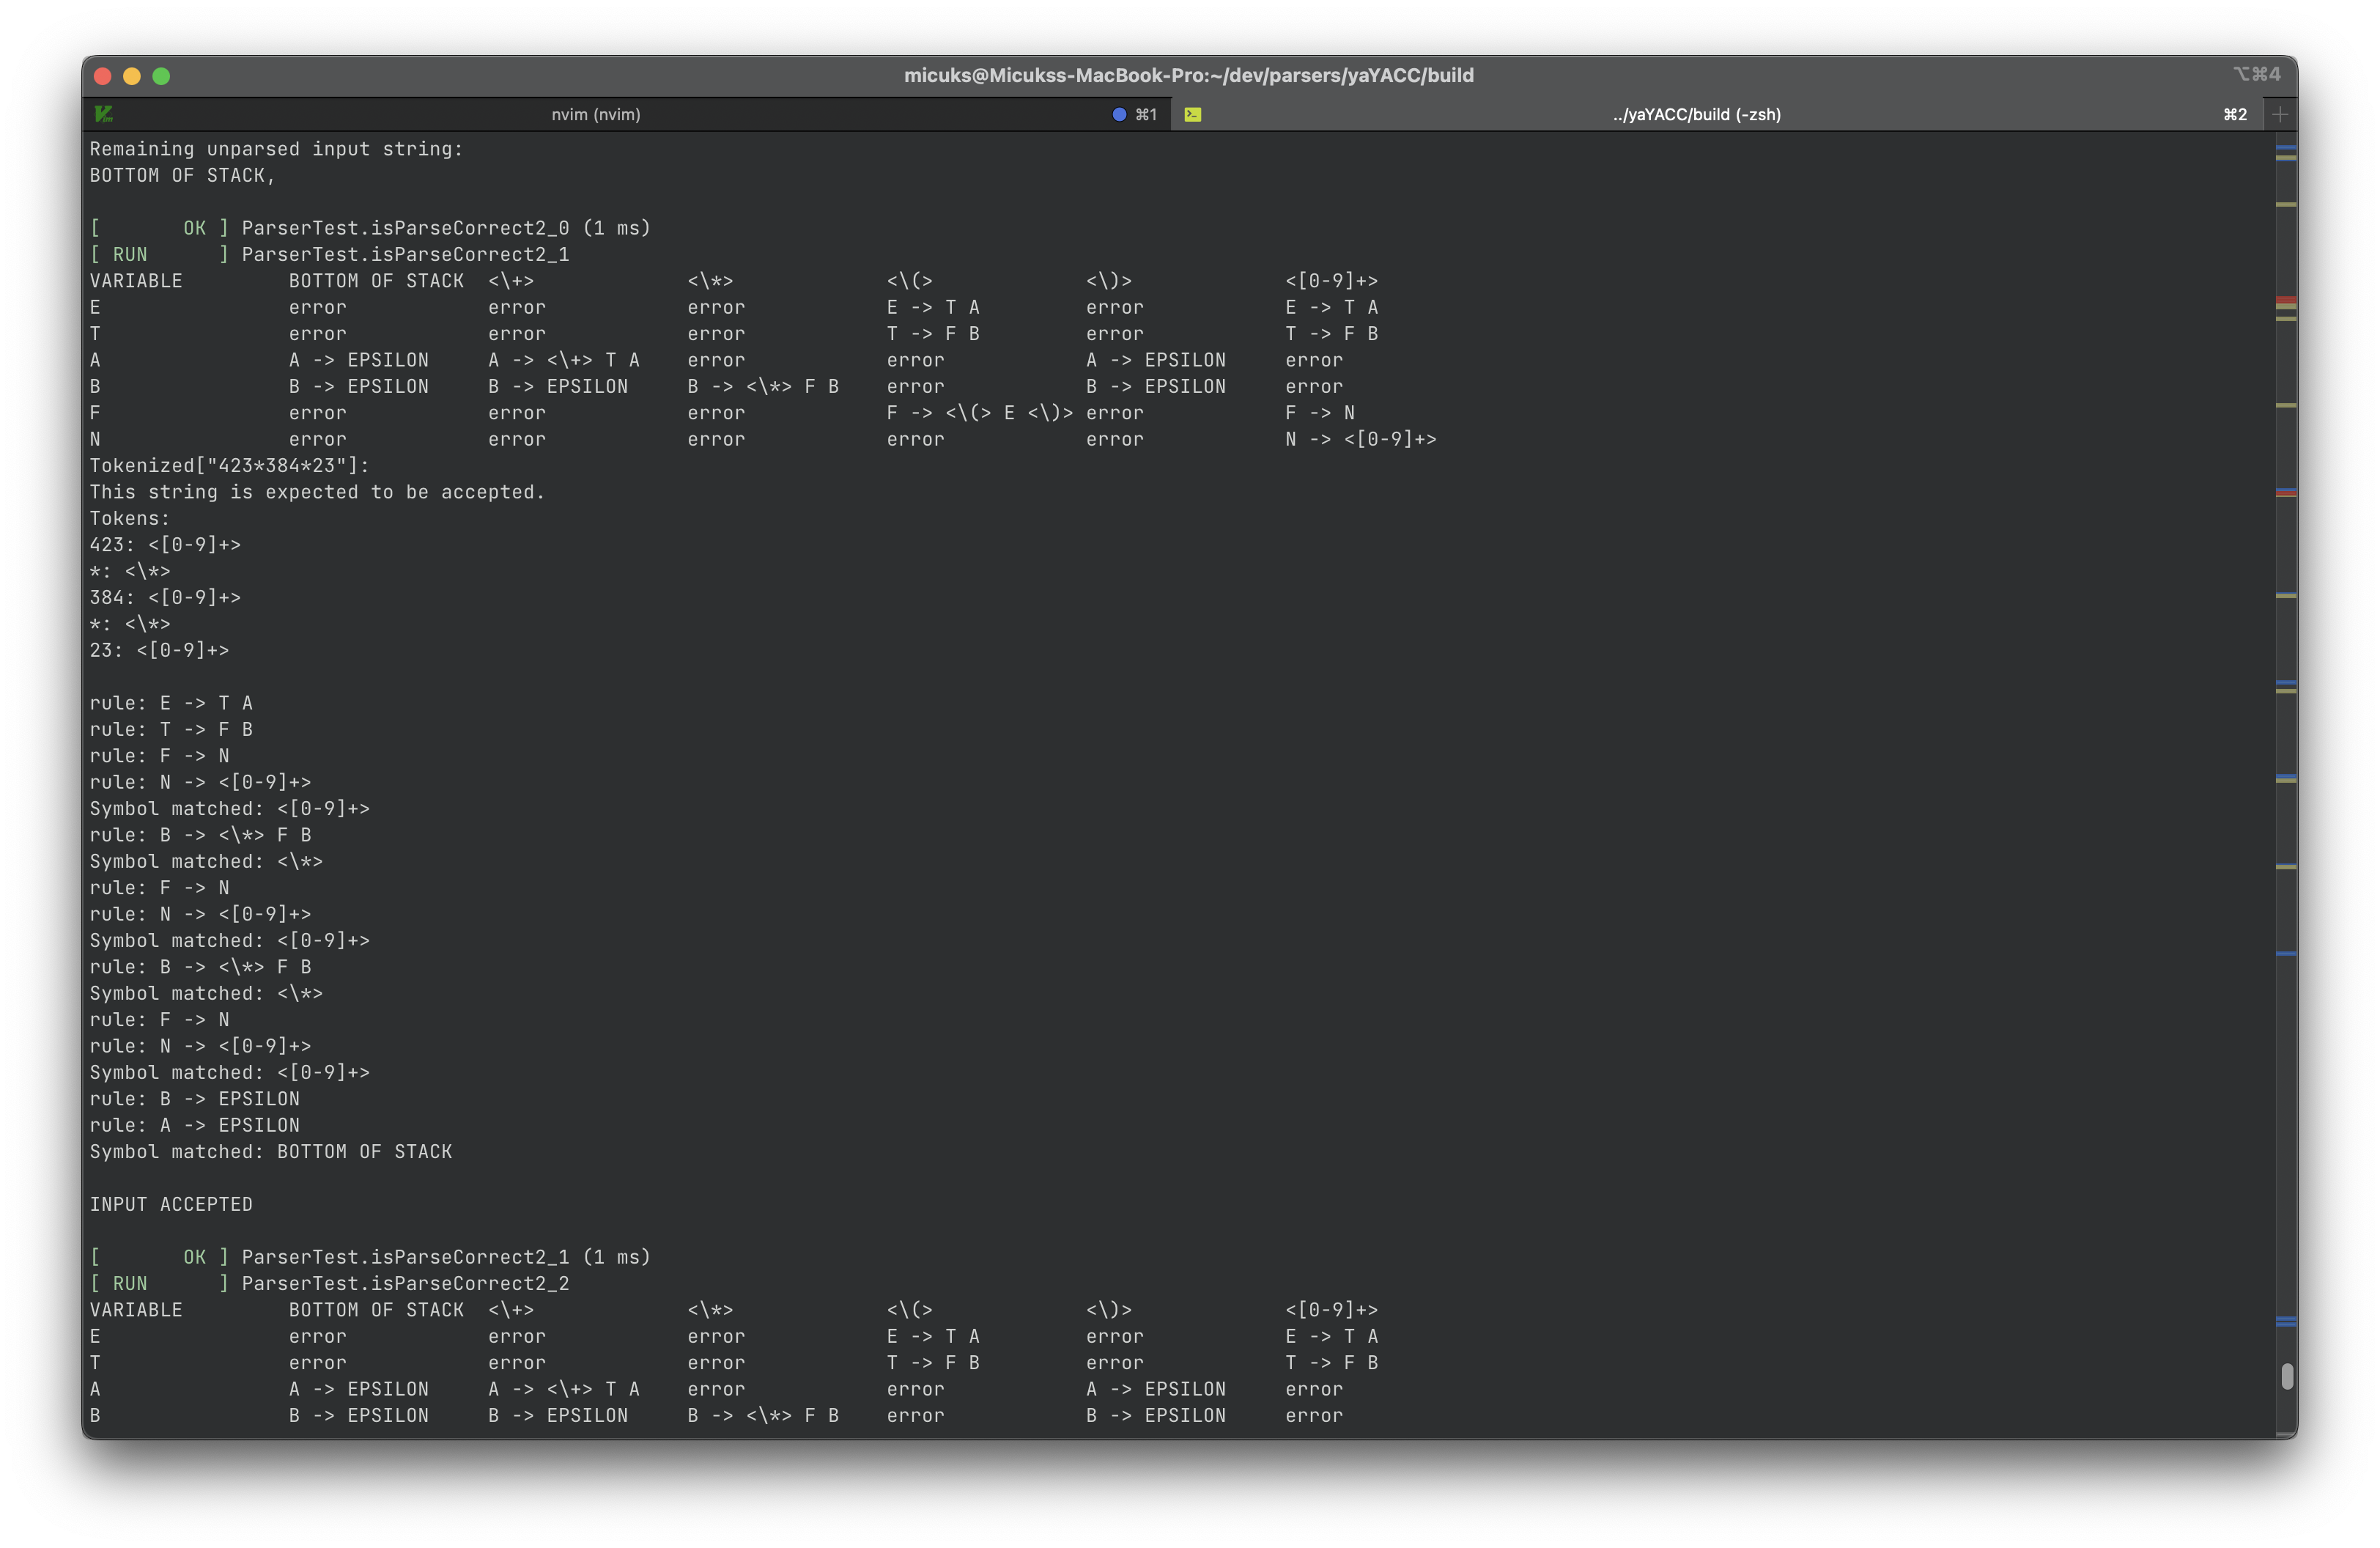
\includegraphics[width=0.95\textwidth]{figures/ll1分析输入21.png}
	\end{center}
	\caption{复杂文法的语法分析}
	\label{fig:复杂文法的语法分析2}
\end{figure}

\subsection{消除左递归测试}
使用作业所给文法作为输入进行测试:
\lstinputlisting[language=c++]{../grammars/g3.txt}

使用多个不同的字符串和文法对LL(1)语法分析程序进行充分测试, 在此不一一展示,
运行日志均放在文末附录.

\subsection{LR(1)语法分析程序}
\subsubsection{生成规范族DFA和LR(1)分析表测试}

首先使用简单的文法进行测试, 文法如下:
\lstinputlisting[language=c++]{../grammars/g1.txt}

测试得到的项目集DFA如图\ref{fig:简单文法的LR1分析测试}LR1 Item Sets部分,
LR(1)分析表如LR1 Parse Table部分,
对输入字符串"  a  b  "进行分析得到的结果紧接在LR1分析表下面, 分析结果为接受.
分析结果氛围三栏, 第一栏为栈, 状态栈和符号栈交叉存储; 第二栏为待分析的tokens,
其中BOTTOM OF STACK为栈底符号, 每个终结符被方括号<>括起; 最后一栏为Action,
表示此时进行的动作, 包括Shift, Reduce, Goto和ACCEPT, 以及出错信息.

\begin{figure}[ht!]
	\begin{center}
		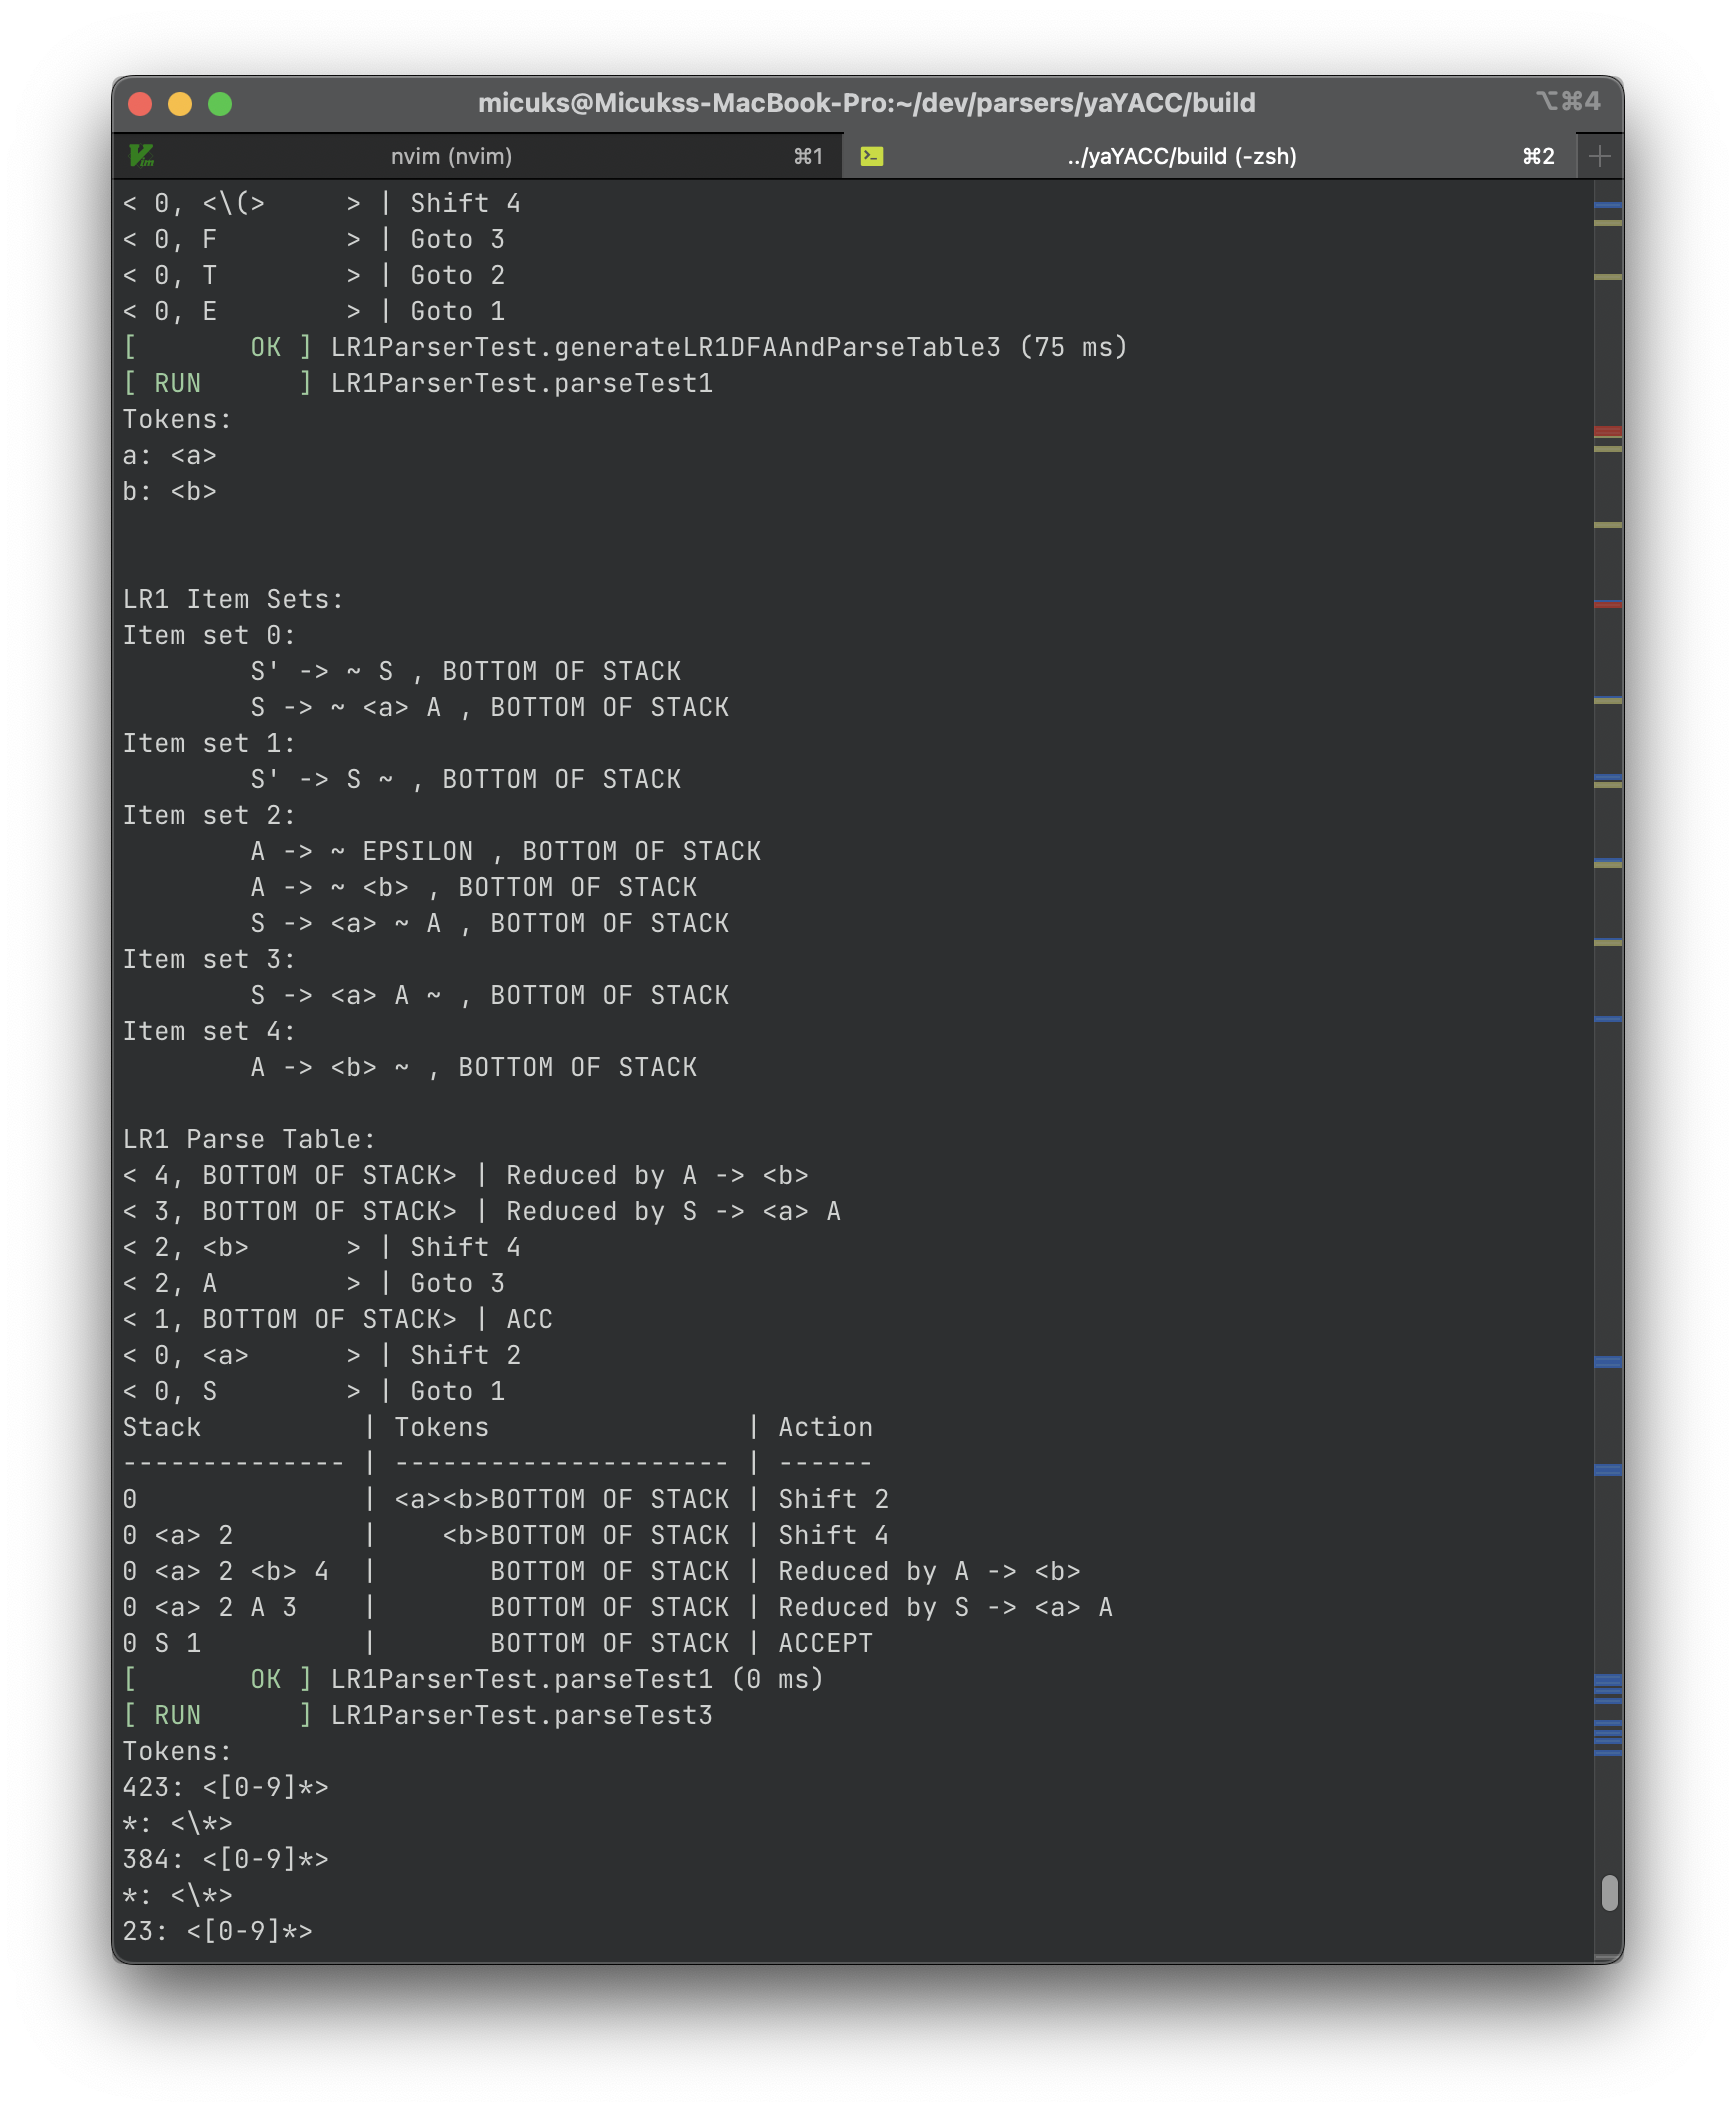
\includegraphics[width=0.95\textwidth]{figures/lr1分析1.png}
	\end{center}
	\caption{简单文法的LR1分析测试}
	\label{fig:简单文法的LR1分析测试}
\end{figure}

然后使用作业所给文法进行测试, 文法如下:
\lstinputlisting[language=c++]{../grammars/g3.txt}

其生成的项目集规范族DFA如下图\ref{fig:复杂文法的LR1项目集规范族DFA}.

\begin{figure}[ht!]
	\begin{center}
		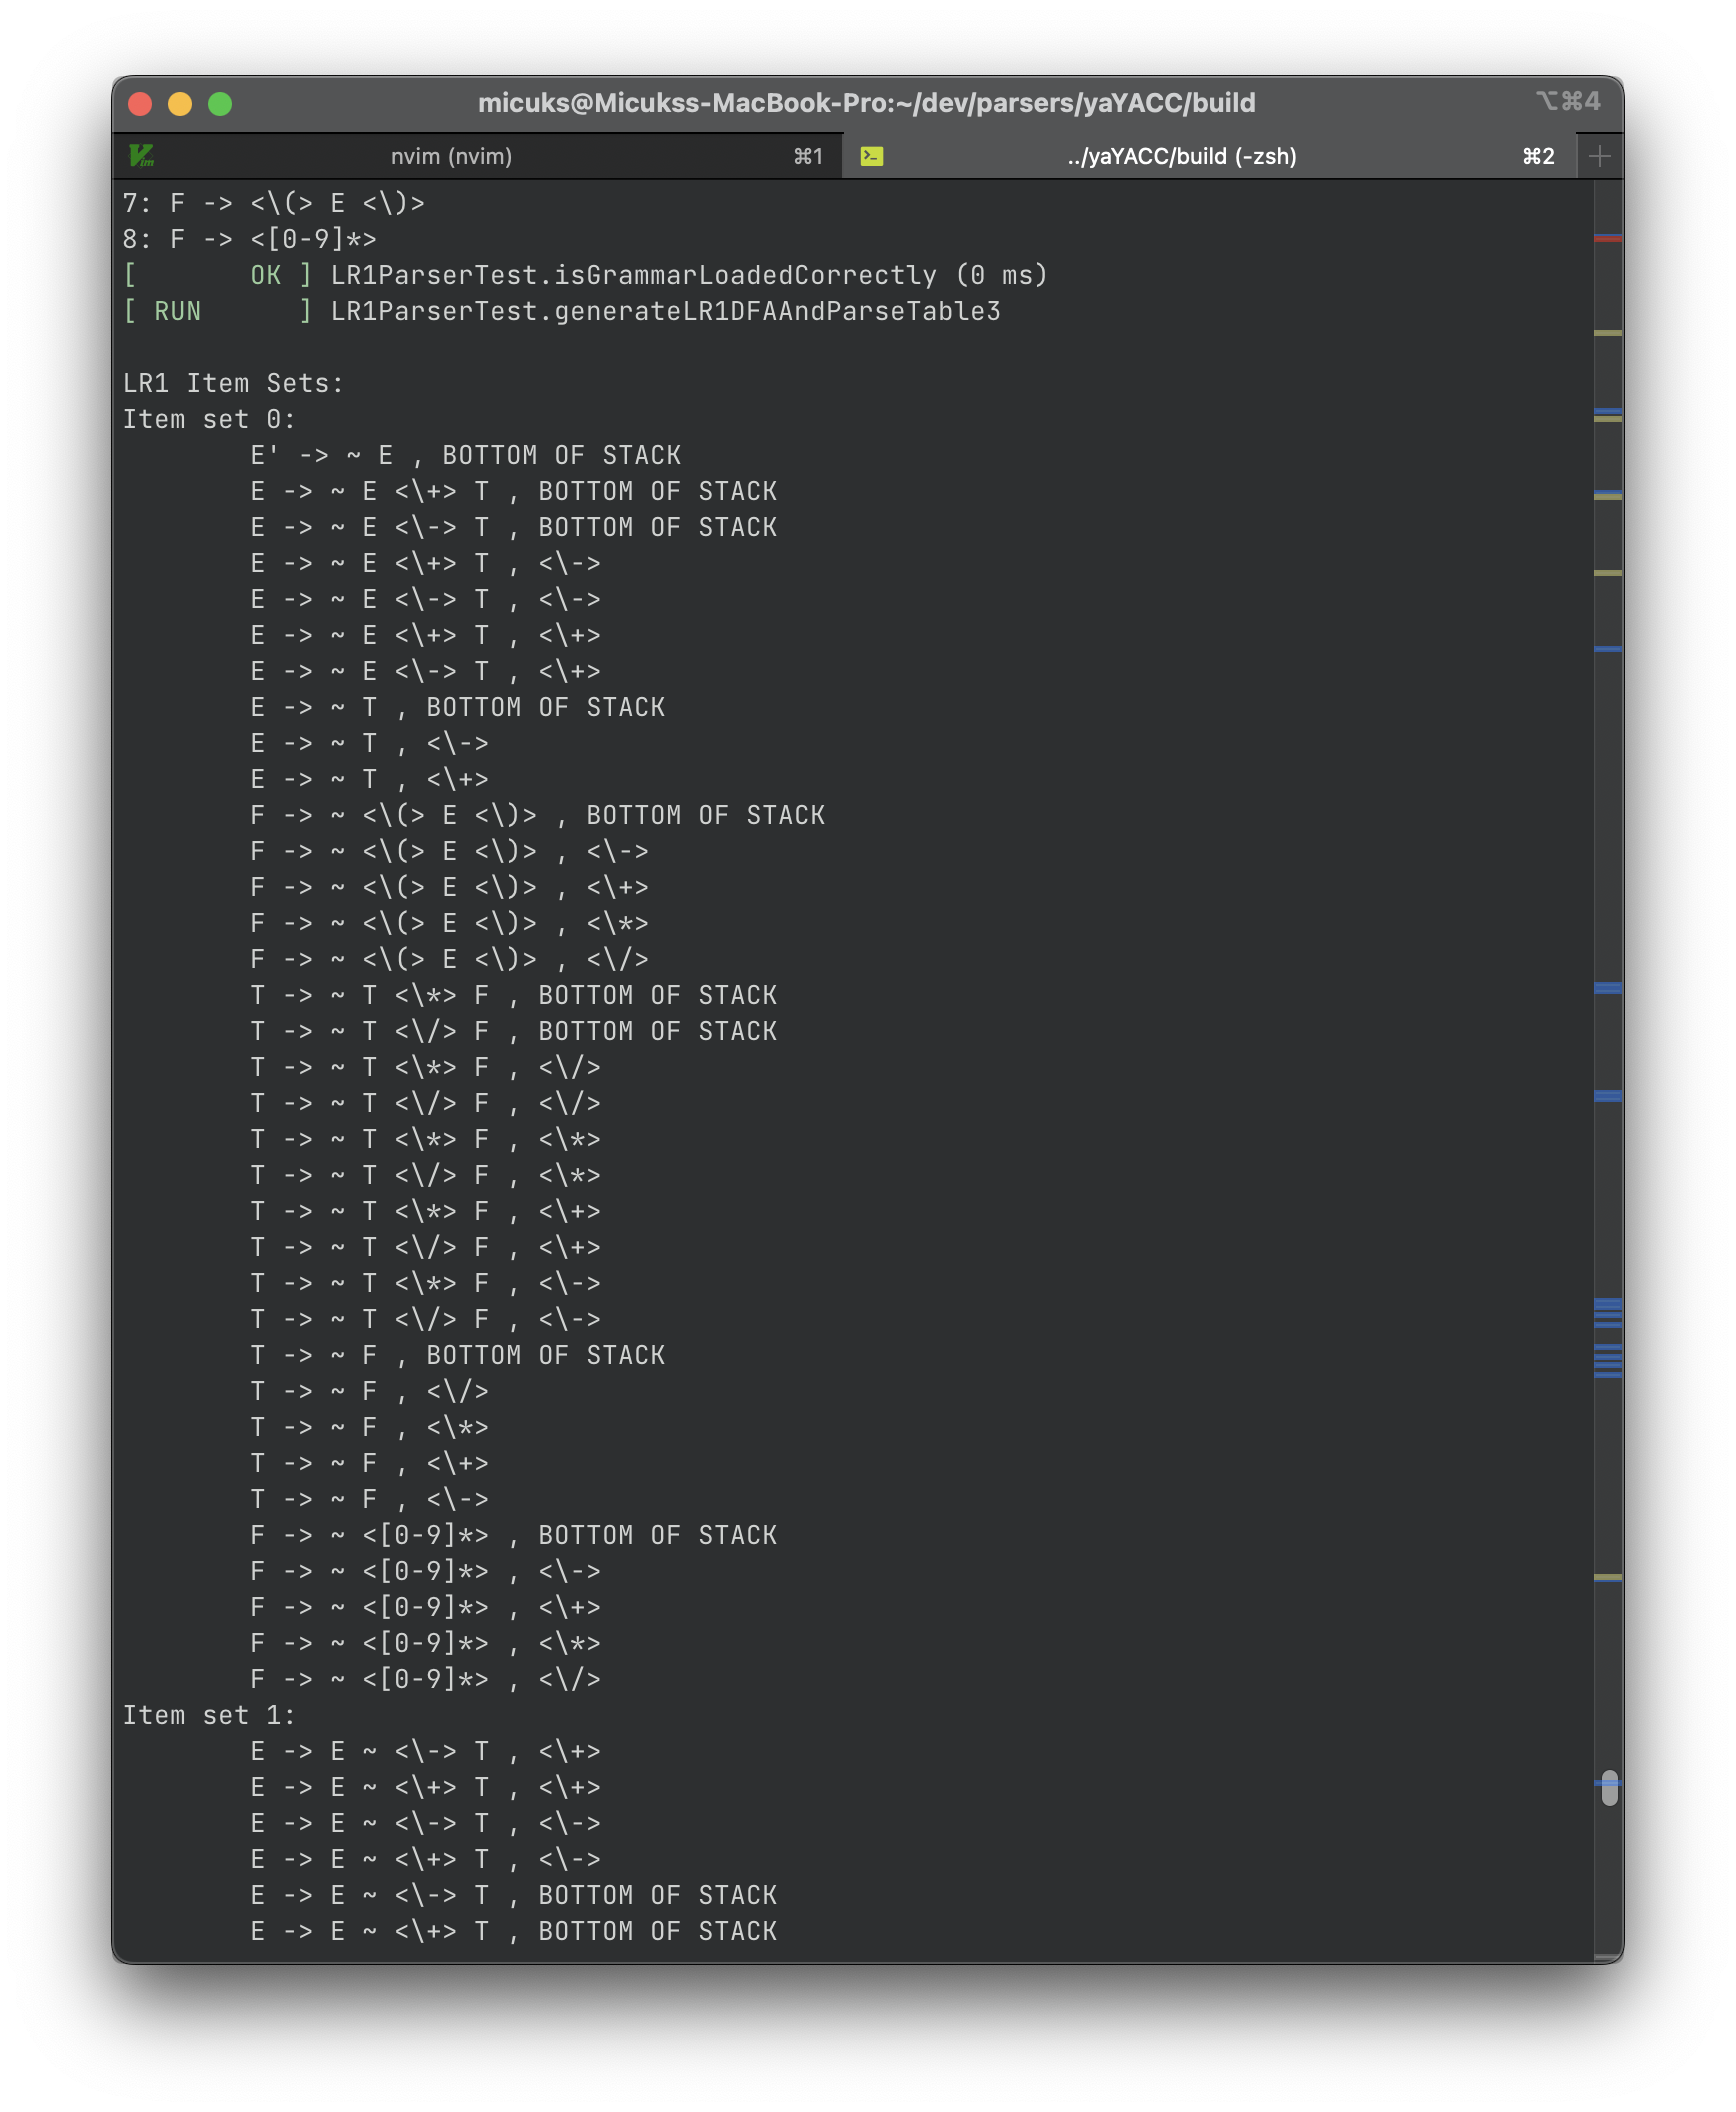
\includegraphics[width=0.95\textwidth]{figures/lr1规范族1.png}
	\end{center}
	\caption{复杂文法的LR1项目集规范族DFA}
	\label{fig:复杂文法的LR1项目集规范族DFA}
\end{figure}

生成的LR1分析表如下图\ref{fig:复杂文法的LR1分析表}:

\begin{figure}[ht!]
	\begin{center}
		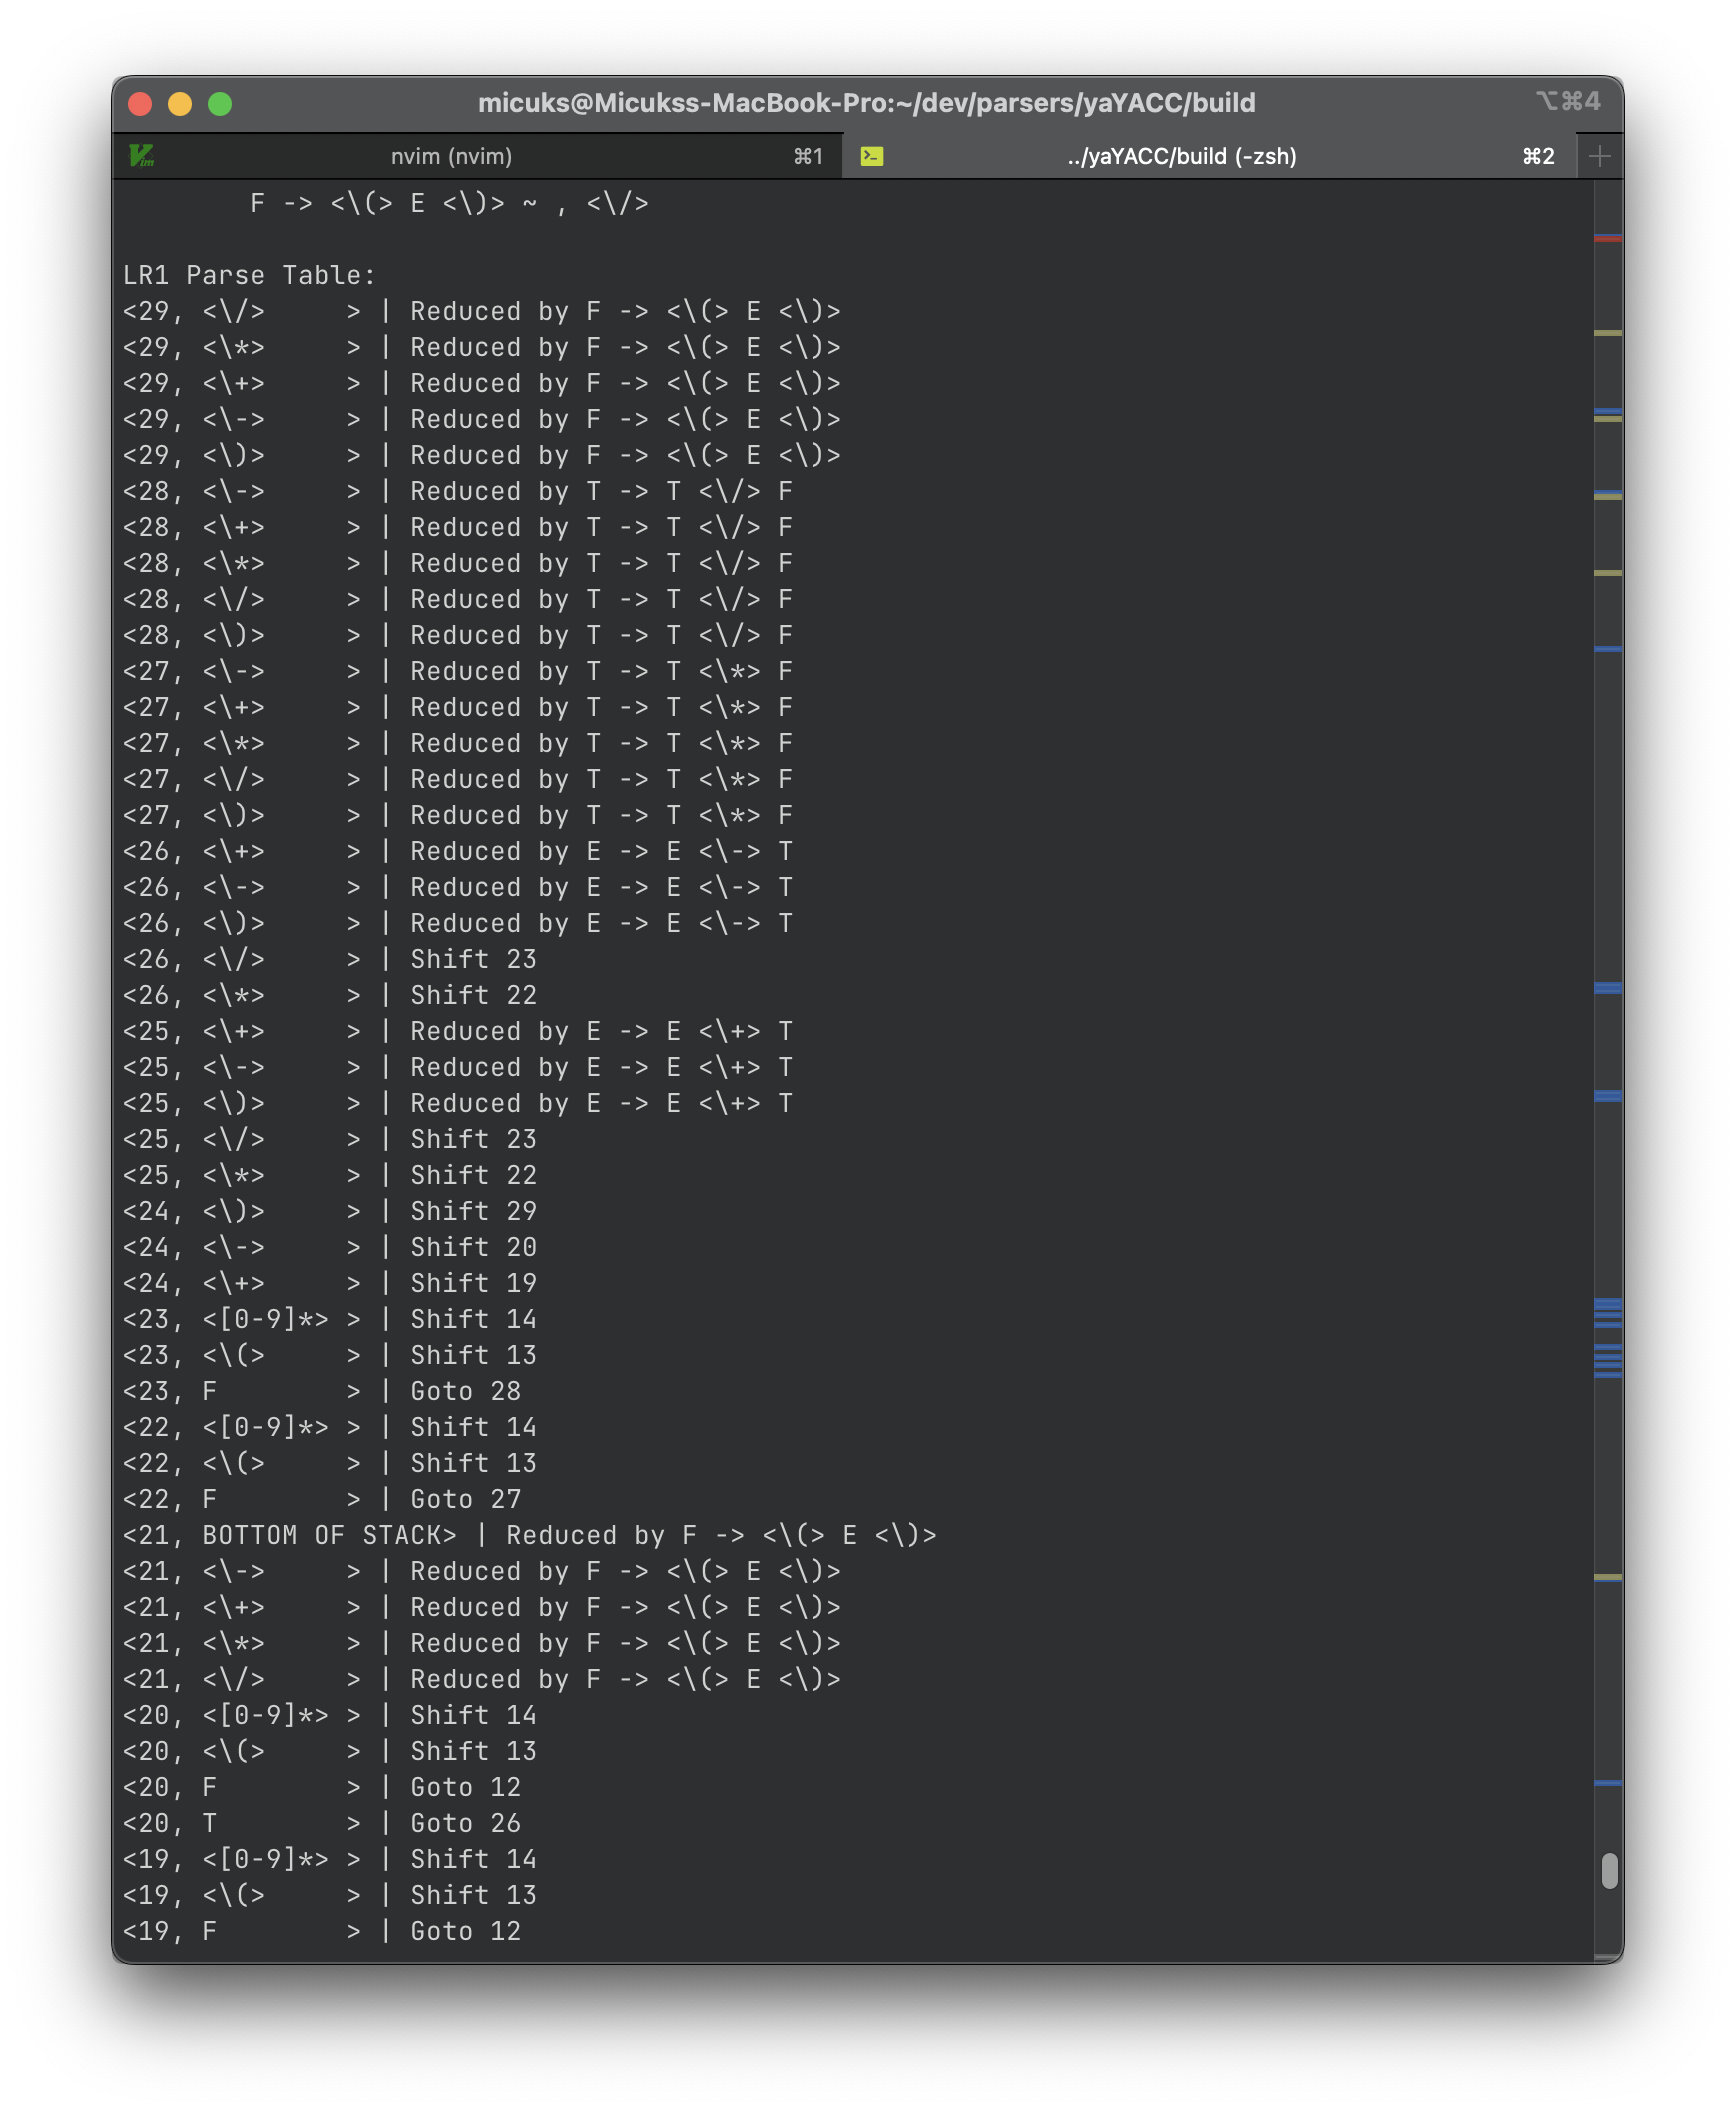
\includegraphics[width=0.95\textwidth]{figures/lr1复杂分析表1.png}
	\end{center}
	\caption{复杂文法的LR1分析表}
	\label{fig:复杂文法的LR1分析表}
\end{figure}

完整DFA和分析表如下.

\begin{lstlisting}[language=c++]
LR1 Item Sets:
Item set 0:
	E' -> ~ E , BOTTOM OF STACK
	E -> ~ E <\+> T , BOTTOM OF STACK
	E -> ~ E <\-> T , BOTTOM OF STACK
	E -> ~ E <\+> T , <\->
	E -> ~ E <\-> T , <\->
	E -> ~ E <\+> T , <\+>
	E -> ~ E <\-> T , <\+>
	E -> ~ T , BOTTOM OF STACK
	E -> ~ T , <\->
	E -> ~ T , <\+>
	T -> ~ T <\*> F , BOTTOM OF STACK
	T -> ~ T <\/> F , BOTTOM OF STACK
	T -> ~ T <\*> F , <\/>
	T -> ~ T <\/> F , <\/>
	T -> ~ T <\*> F , <\*>
	T -> ~ T <\/> F , <\*>
	T -> ~ T <\*> F , <\+>
	T -> ~ T <\/> F , <\+>
	T -> ~ T <\*> F , <\->
	T -> ~ T <\/> F , <\->
	T -> ~ F , BOTTOM OF STACK
	T -> ~ F , <\/>
	T -> ~ F , <\*>
	T -> ~ F , <\+>
	T -> ~ F , <\->
	F -> ~ <\(> E <\)> , BOTTOM OF STACK
	F -> ~ <\(> E <\)> , <\->
	F -> ~ <\(> E <\)> , <\+>
	F -> ~ <\(> E <\)> , <\*>
	F -> ~ <\(> E <\)> , <\/>
	F -> ~ <[0-9]*> , BOTTOM OF STACK
	F -> ~ <[0-9]*> , <\->
	F -> ~ <[0-9]*> , <\+>
	F -> ~ <[0-9]*> , <\*>
	F -> ~ <[0-9]*> , <\/>
Item set 1:
	E -> E ~ <\-> T , <\+>
	E -> E ~ <\+> T , <\+>
	E -> E ~ <\-> T , <\->
	E -> E ~ <\+> T , <\->
	E -> E ~ <\-> T , BOTTOM OF STACK
	E -> E ~ <\+> T , BOTTOM OF STACK
	E' -> E ~ , BOTTOM OF STACK
Item set 2:
	T -> T ~ <\/> F , <\->
	T -> T ~ <\*> F , <\->
	T -> T ~ <\/> F , <\+>
	T -> T ~ <\*> F , <\+>
	T -> T ~ <\/> F , <\*>
	T -> T ~ <\*> F , <\*>
	T -> T ~ <\/> F , <\/>
	T -> T ~ <\*> F , <\/>
	T -> T ~ <\/> F , BOTTOM OF STACK
	T -> T ~ <\*> F , BOTTOM OF STACK
	E -> T ~ , <\+>
	E -> T ~ , <\->
	E -> T ~ , BOTTOM OF STACK
Item set 3:
	T -> F ~ , <\->
	T -> F ~ , <\+>
	T -> F ~ , <\*>
	T -> F ~ , <\/>
	T -> F ~ , BOTTOM OF STACK
Item set 4:
	F -> ~ <[0-9]*> , <\/>
	F -> ~ <[0-9]*> , <\*>
	F -> ~ <[0-9]*> , <\+>
	F -> ~ <[0-9]*> , <\->
	F -> ~ <[0-9]*> , <\)>
	F -> ~ <\(> E <\)> , <\/>
	F -> ~ <\(> E <\)> , <\*>
	F -> ~ <\(> E <\)> , <\+>
	F -> ~ <\(> E <\)> , <\->
	F -> ~ <\(> E <\)> , <\)>
	T -> ~ T <\/> F , <\->
	T -> ~ T <\*> F , <\->
	T -> ~ T <\/> F , <\+>
	T -> ~ T <\*> F , <\+>
	T -> ~ T <\/> F , <\*>
	T -> ~ T <\*> F , <\*>
	T -> ~ T <\/> F , <\/>
	T -> ~ T <\*> F , <\/>
	T -> ~ T <\/> F , <\)>
	T -> ~ T <\*> F , <\)>
	E -> ~ T , <\+>
	E -> ~ T , <\->
	E -> ~ T , <\)>
	E -> ~ E <\-> T , <\+>
	E -> ~ E <\+> T , <\+>
	E -> ~ E <\-> T , <\->
	E -> ~ E <\+> T , <\->
	E -> ~ E <\-> T , <\)>
	E -> ~ E <\+> T , <\)>
	T -> ~ F , <\->
	T -> ~ F , <\+>
	T -> ~ F , <\*>
	T -> ~ F , <\/>
	T -> ~ F , <\)>
	F -> <\(> ~ E <\)> , <\/>
	F -> <\(> ~ E <\)> , <\*>
	F -> <\(> ~ E <\)> , <\+>
	F -> <\(> ~ E <\)> , <\->
	F -> <\(> ~ E <\)> , BOTTOM OF STACK
Item set 5:
	F -> <[0-9]*> ~ , <\/>
	F -> <[0-9]*> ~ , <\*>
	F -> <[0-9]*> ~ , <\+>
	F -> <[0-9]*> ~ , <\->
	F -> <[0-9]*> ~ , BOTTOM OF STACK
Item set 6:
	F -> ~ <[0-9]*> , <\/>
	F -> ~ <[0-9]*> , <\*>
	F -> ~ <[0-9]*> , BOTTOM OF STACK
	F -> ~ <[0-9]*> , <\->
	F -> ~ <[0-9]*> , <\+>
	F -> ~ <\(> E <\)> , <\/>
	F -> ~ <\(> E <\)> , <\*>
	F -> ~ <\(> E <\)> , BOTTOM OF STACK
	F -> ~ <\(> E <\)> , <\->
	F -> ~ <\(> E <\)> , <\+>
	T -> ~ F , <\*>
	T -> ~ F , <\/>
	T -> ~ F , <\+>
	T -> ~ F , <\->
	T -> ~ F , BOTTOM OF STACK
	T -> ~ T <\/> F , <\*>
	T -> ~ T <\*> F , <\*>
	T -> ~ T <\/> F , <\/>
	T -> ~ T <\*> F , <\/>
	T -> ~ T <\/> F , <\+>
	T -> ~ T <\*> F , <\+>
	T -> ~ T <\/> F , <\->
	T -> ~ T <\*> F , <\->
	T -> ~ T <\/> F , BOTTOM OF STACK
	T -> ~ T <\*> F , BOTTOM OF STACK
	E -> E <\+> ~ T , BOTTOM OF STACK
	E -> E <\+> ~ T , <\->
	E -> E <\+> ~ T , <\+>
Item set 7:
	F -> ~ <[0-9]*> , <\/>
	F -> ~ <[0-9]*> , <\*>
	F -> ~ <[0-9]*> , BOTTOM OF STACK
	F -> ~ <[0-9]*> , <\->
	F -> ~ <[0-9]*> , <\+>
	F -> ~ <\(> E <\)> , <\/>
	F -> ~ <\(> E <\)> , <\*>
	F -> ~ <\(> E <\)> , BOTTOM OF STACK
	F -> ~ <\(> E <\)> , <\->
	F -> ~ <\(> E <\)> , <\+>
	T -> ~ F , <\*>
	T -> ~ F , <\/>
	T -> ~ F , <\+>
	T -> ~ F , <\->
	T -> ~ F , BOTTOM OF STACK
	T -> ~ T <\/> F , <\*>
	T -> ~ T <\*> F , <\*>
	T -> ~ T <\/> F , <\/>
	T -> ~ T <\*> F , <\/>
	T -> ~ T <\/> F , <\+>
	T -> ~ T <\*> F , <\+>
	T -> ~ T <\/> F , <\->
	T -> ~ T <\*> F , <\->
	T -> ~ T <\/> F , BOTTOM OF STACK
	T -> ~ T <\*> F , BOTTOM OF STACK
	E -> E <\-> ~ T , BOTTOM OF STACK
	E -> E <\-> ~ T , <\->
	E -> E <\-> ~ T , <\+>
Item set 8:
	F -> ~ <[0-9]*> , <\->
	F -> ~ <[0-9]*> , <\+>
	F -> ~ <[0-9]*> , <\*>
	F -> ~ <[0-9]*> , <\/>
	F -> ~ <[0-9]*> , BOTTOM OF STACK
	F -> ~ <\(> E <\)> , <\->
	F -> ~ <\(> E <\)> , <\+>
	F -> ~ <\(> E <\)> , <\*>
	F -> ~ <\(> E <\)> , <\/>
	F -> ~ <\(> E <\)> , BOTTOM OF STACK
	T -> T <\*> ~ F , BOTTOM OF STACK
	T -> T <\*> ~ F , <\/>
	T -> T <\*> ~ F , <\*>
	T -> T <\*> ~ F , <\+>
	T -> T <\*> ~ F , <\->
Item set 9:
	F -> ~ <[0-9]*> , <\->
	F -> ~ <[0-9]*> , <\+>
	F -> ~ <[0-9]*> , <\*>
	F -> ~ <[0-9]*> , <\/>
	F -> ~ <[0-9]*> , BOTTOM OF STACK
	F -> ~ <\(> E <\)> , <\->
	F -> ~ <\(> E <\)> , <\+>
	F -> ~ <\(> E <\)> , <\*>
	F -> ~ <\(> E <\)> , <\/>
	F -> ~ <\(> E <\)> , BOTTOM OF STACK
	T -> T <\/> ~ F , BOTTOM OF STACK
	T -> T <\/> ~ F , <\/>
	T -> T <\/> ~ F , <\*>
	T -> T <\/> ~ F , <\+>
	T -> T <\/> ~ F , <\->
Item set 10:
	F -> <\(> E ~ <\)> , BOTTOM OF STACK
	F -> <\(> E ~ <\)> , <\->
	F -> <\(> E ~ <\)> , <\+>
	F -> <\(> E ~ <\)> , <\*>
	F -> <\(> E ~ <\)> , <\/>
	E -> E ~ <\+> T , <\)>
	E -> E ~ <\-> T , <\)>
	E -> E ~ <\+> T , <\->
	E -> E ~ <\-> T , <\->
	E -> E ~ <\+> T , <\+>
	E -> E ~ <\-> T , <\+>
Item set 11:
	E -> T ~ , <\)>
	E -> T ~ , <\->
	E -> T ~ , <\+>
	T -> T ~ <\*> F , <\)>
	T -> T ~ <\/> F , <\)>
	T -> T ~ <\*> F , <\/>
	T -> T ~ <\/> F , <\/>
	T -> T ~ <\*> F , <\*>
	T -> T ~ <\/> F , <\*>
	T -> T ~ <\*> F , <\+>
	T -> T ~ <\/> F , <\+>
	T -> T ~ <\*> F , <\->
	T -> T ~ <\/> F , <\->
Item set 12:
	T -> F ~ , <\)>
	T -> F ~ , <\/>
	T -> F ~ , <\*>
	T -> F ~ , <\+>
	T -> F ~ , <\->
Item set 13:
	F -> ~ <[0-9]*> , <\/>
	F -> ~ <[0-9]*> , <\*>
	F -> ~ <[0-9]*> , <\+>
	F -> ~ <[0-9]*> , <\->
	F -> ~ <[0-9]*> , <\)>
	F -> ~ <\(> E <\)> , <\/>
	F -> ~ <\(> E <\)> , <\*>
	F -> ~ <\(> E <\)> , <\+>
	F -> ~ <\(> E <\)> , <\->
	F -> ~ <\(> E <\)> , <\)>
	T -> ~ T <\/> F , <\->
	T -> ~ T <\*> F , <\->
	T -> ~ T <\/> F , <\+>
	T -> ~ T <\*> F , <\+>
	T -> ~ T <\/> F , <\*>
	T -> ~ T <\*> F , <\*>
	T -> ~ T <\/> F , <\/>
	T -> ~ T <\*> F , <\/>
	T -> ~ T <\/> F , <\)>
	T -> ~ T <\*> F , <\)>
	E -> ~ T , <\+>
	E -> ~ T , <\->
	E -> ~ T , <\)>
	E -> ~ E <\-> T , <\+>
	E -> ~ E <\+> T , <\+>
	E -> ~ E <\-> T , <\->
	E -> ~ E <\+> T , <\->
	E -> ~ E <\-> T , <\)>
	E -> ~ E <\+> T , <\)>
	T -> ~ F , <\->
	T -> ~ F , <\+>
	T -> ~ F , <\*>
	T -> ~ F , <\/>
	T -> ~ F , <\)>
	F -> <\(> ~ E <\)> , <\)>
	F -> <\(> ~ E <\)> , <\->
	F -> <\(> ~ E <\)> , <\+>
	F -> <\(> ~ E <\)> , <\*>
	F -> <\(> ~ E <\)> , <\/>
Item set 14:
	F -> <[0-9]*> ~ , <\)>
	F -> <[0-9]*> ~ , <\->
	F -> <[0-9]*> ~ , <\+>
	F -> <[0-9]*> ~ , <\*>
	F -> <[0-9]*> ~ , <\/>
Item set 15:
	E -> E <\+> T ~ , <\+>
	E -> E <\+> T ~ , <\->
	E -> E <\+> T ~ , BOTTOM OF STACK
	T -> T ~ <\*> F , BOTTOM OF STACK
	T -> T ~ <\/> F , BOTTOM OF STACK
	T -> T ~ <\*> F , <\->
	T -> T ~ <\/> F , <\->
	T -> T ~ <\*> F , <\+>
	T -> T ~ <\/> F , <\+>
	T -> T ~ <\*> F , <\/>
	T -> T ~ <\/> F , <\/>
	T -> T ~ <\*> F , <\*>
	T -> T ~ <\/> F , <\*>
Item set 16:
	E -> E <\-> T ~ , <\+>
	E -> E <\-> T ~ , <\->
	E -> E <\-> T ~ , BOTTOM OF STACK
	T -> T ~ <\*> F , BOTTOM OF STACK
	T -> T ~ <\/> F , BOTTOM OF STACK
	T -> T ~ <\*> F , <\->
	T -> T ~ <\/> F , <\->
	T -> T ~ <\*> F , <\+>
	T -> T ~ <\/> F , <\+>
	T -> T ~ <\*> F , <\/>
	T -> T ~ <\/> F , <\/>
	T -> T ~ <\*> F , <\*>
	T -> T ~ <\/> F , <\*>
Item set 17:
	T -> T <\*> F ~ , <\->
	T -> T <\*> F ~ , <\+>
	T -> T <\*> F ~ , <\*>
	T -> T <\*> F ~ , <\/>
	T -> T <\*> F ~ , BOTTOM OF STACK
Item set 18:
	T -> T <\/> F ~ , <\->
	T -> T <\/> F ~ , <\+>
	T -> T <\/> F ~ , <\*>
	T -> T <\/> F ~ , <\/>
	T -> T <\/> F ~ , BOTTOM OF STACK
Item set 19:
	F -> ~ <[0-9]*> , <\/>
	F -> ~ <[0-9]*> , <\*>
	F -> ~ <[0-9]*> , <\+>
	F -> ~ <[0-9]*> , <\->
	F -> ~ <[0-9]*> , <\)>
	F -> ~ <\(> E <\)> , <\/>
	F -> ~ <\(> E <\)> , <\*>
	F -> ~ <\(> E <\)> , <\+>
	F -> ~ <\(> E <\)> , <\->
	F -> ~ <\(> E <\)> , <\)>
	T -> ~ F , <\*>
	T -> ~ F , <\/>
	T -> ~ F , <\)>
	T -> ~ F , <\->
	T -> ~ F , <\+>
	T -> ~ T <\/> F , <\*>
	T -> ~ T <\*> F , <\*>
	T -> ~ T <\/> F , <\/>
	T -> ~ T <\*> F , <\/>
	T -> ~ T <\/> F , <\)>
	T -> ~ T <\*> F , <\)>
	T -> ~ T <\/> F , <\->
	T -> ~ T <\*> F , <\->
	T -> ~ T <\/> F , <\+>
	T -> ~ T <\*> F , <\+>
	E -> E <\+> ~ T , <\+>
	E -> E <\+> ~ T , <\->
	E -> E <\+> ~ T , <\)>
Item set 20:
	F -> ~ <[0-9]*> , <\/>
	F -> ~ <[0-9]*> , <\*>
	F -> ~ <[0-9]*> , <\+>
	F -> ~ <[0-9]*> , <\->
	F -> ~ <[0-9]*> , <\)>
	F -> ~ <\(> E <\)> , <\/>
	F -> ~ <\(> E <\)> , <\*>
	F -> ~ <\(> E <\)> , <\+>
	F -> ~ <\(> E <\)> , <\->
	F -> ~ <\(> E <\)> , <\)>
	T -> ~ F , <\*>
	T -> ~ F , <\/>
	T -> ~ F , <\)>
	T -> ~ F , <\->
	T -> ~ F , <\+>
	T -> ~ T <\/> F , <\*>
	T -> ~ T <\*> F , <\*>
	T -> ~ T <\/> F , <\/>
	T -> ~ T <\*> F , <\/>
	T -> ~ T <\/> F , <\)>
	T -> ~ T <\*> F , <\)>
	T -> ~ T <\/> F , <\->
	T -> ~ T <\*> F , <\->
	T -> ~ T <\/> F , <\+>
	T -> ~ T <\*> F , <\+>
	E -> E <\-> ~ T , <\+>
	E -> E <\-> ~ T , <\->
	E -> E <\-> ~ T , <\)>
Item set 21:
	F -> <\(> E <\)> ~ , <\/>
	F -> <\(> E <\)> ~ , <\*>
	F -> <\(> E <\)> ~ , <\+>
	F -> <\(> E <\)> ~ , <\->
	F -> <\(> E <\)> ~ , BOTTOM OF STACK
Item set 22:
	F -> ~ <[0-9]*> , <\)>
	F -> ~ <[0-9]*> , <\/>
	F -> ~ <[0-9]*> , <\*>
	F -> ~ <[0-9]*> , <\+>
	F -> ~ <[0-9]*> , <\->
	F -> ~ <\(> E <\)> , <\)>
	F -> ~ <\(> E <\)> , <\/>
	F -> ~ <\(> E <\)> , <\*>
	F -> ~ <\(> E <\)> , <\+>
	F -> ~ <\(> E <\)> , <\->
	T -> T <\*> ~ F , <\->
	T -> T <\*> ~ F , <\+>
	T -> T <\*> ~ F , <\*>
	T -> T <\*> ~ F , <\/>
	T -> T <\*> ~ F , <\)>
Item set 23:
	F -> ~ <[0-9]*> , <\)>
	F -> ~ <[0-9]*> , <\/>
	F -> ~ <[0-9]*> , <\*>
	F -> ~ <[0-9]*> , <\+>
	F -> ~ <[0-9]*> , <\->
	F -> ~ <\(> E <\)> , <\)>
	F -> ~ <\(> E <\)> , <\/>
	F -> ~ <\(> E <\)> , <\*>
	F -> ~ <\(> E <\)> , <\+>
	F -> ~ <\(> E <\)> , <\->
	T -> T <\/> ~ F , <\->
	T -> T <\/> ~ F , <\+>
	T -> T <\/> ~ F , <\*>
	T -> T <\/> ~ F , <\/>
	T -> T <\/> ~ F , <\)>
Item set 24:
	F -> <\(> E ~ <\)> , <\/>
	F -> <\(> E ~ <\)> , <\*>
	F -> <\(> E ~ <\)> , <\+>
	F -> <\(> E ~ <\)> , <\->
	F -> <\(> E ~ <\)> , <\)>
	E -> E ~ <\+> T , <\)>
	E -> E ~ <\-> T , <\)>
	E -> E ~ <\+> T , <\->
	E -> E ~ <\-> T , <\->
	E -> E ~ <\+> T , <\+>
	E -> E ~ <\-> T , <\+>
Item set 25:
	E -> E <\+> T ~ , <\)>
	E -> E <\+> T ~ , <\->
	E -> E <\+> T ~ , <\+>
	T -> T ~ <\*> F , <\+>
	T -> T ~ <\/> F , <\+>
	T -> T ~ <\*> F , <\->
	T -> T ~ <\/> F , <\->
	T -> T ~ <\*> F , <\)>
	T -> T ~ <\/> F , <\)>
	T -> T ~ <\*> F , <\/>
	T -> T ~ <\/> F , <\/>
	T -> T ~ <\*> F , <\*>
	T -> T ~ <\/> F , <\*>
Item set 26:
	E -> E <\-> T ~ , <\)>
	E -> E <\-> T ~ , <\->
	E -> E <\-> T ~ , <\+>
	T -> T ~ <\*> F , <\+>
	T -> T ~ <\/> F , <\+>
	T -> T ~ <\*> F , <\->
	T -> T ~ <\/> F , <\->
	T -> T ~ <\*> F , <\)>
	T -> T ~ <\/> F , <\)>
	T -> T ~ <\*> F , <\/>
	T -> T ~ <\/> F , <\/>
	T -> T ~ <\*> F , <\*>
	T -> T ~ <\/> F , <\*>
Item set 27:
	T -> T <\*> F ~ , <\)>
	T -> T <\*> F ~ , <\/>
	T -> T <\*> F ~ , <\*>
	T -> T <\*> F ~ , <\+>
	T -> T <\*> F ~ , <\->
Item set 28:
	T -> T <\/> F ~ , <\)>
	T -> T <\/> F ~ , <\/>
	T -> T <\/> F ~ , <\*>
	T -> T <\/> F ~ , <\+>
	T -> T <\/> F ~ , <\->
Item set 29:
	F -> <\(> E <\)> ~ , <\)>
	F -> <\(> E <\)> ~ , <\->
	F -> <\(> E <\)> ~ , <\+>
	F -> <\(> E <\)> ~ , <\*>
	F -> <\(> E <\)> ~ , <\/>

LR1 Parse Table:
<29, <\/>     > | Reduced by F -> <\(> E <\)>
<29, <\*>     > | Reduced by F -> <\(> E <\)>
<29, <\+>     > | Reduced by F -> <\(> E <\)>
<29, <\->     > | Reduced by F -> <\(> E <\)>
<29, <\)>     > | Reduced by F -> <\(> E <\)>
<28, <\->     > | Reduced by T -> T <\/> F
<28, <\+>     > | Reduced by T -> T <\/> F
<28, <\*>     > | Reduced by T -> T <\/> F
<28, <\/>     > | Reduced by T -> T <\/> F
<28, <\)>     > | Reduced by T -> T <\/> F
<27, <\->     > | Reduced by T -> T <\*> F
<27, <\+>     > | Reduced by T -> T <\*> F
<27, <\*>     > | Reduced by T -> T <\*> F
<27, <\/>     > | Reduced by T -> T <\*> F
<27, <\)>     > | Reduced by T -> T <\*> F
<26, <\+>     > | Reduced by E -> E <\-> T
<26, <\->     > | Reduced by E -> E <\-> T
<26, <\)>     > | Reduced by E -> E <\-> T
<26, <\/>     > | Shift 23
<26, <\*>     > | Shift 22
<25, <\+>     > | Reduced by E -> E <\+> T
<25, <\->     > | Reduced by E -> E <\+> T
<25, <\)>     > | Reduced by E -> E <\+> T
<25, <\/>     > | Shift 23
<25, <\*>     > | Shift 22
<24, <\)>     > | Shift 29
<24, <\->     > | Shift 20
<24, <\+>     > | Shift 19
<23, <[0-9]*> > | Shift 14
<23, <\(>     > | Shift 13
<23, F        > | Goto 28
<22, <[0-9]*> > | Shift 14
<22, <\(>     > | Shift 13
<22, F        > | Goto 27
<21, BOTTOM OF STACK> | Reduced by F -> <\(> E <\)>
<21, <\->     > | Reduced by F -> <\(> E <\)>
<21, <\+>     > | Reduced by F -> <\(> E <\)>
<21, <\*>     > | Reduced by F -> <\(> E <\)>
<21, <\/>     > | Reduced by F -> <\(> E <\)>
<20, <[0-9]*> > | Shift 14
<20, <\(>     > | Shift 13
<20, F        > | Goto 12
<20, T        > | Goto 26
<19, <[0-9]*> > | Shift 14
<19, <\(>     > | Shift 13
<19, F        > | Goto 12
<19, T        > | Goto 25
<18, BOTTOM OF STACK> | Reduced by T -> T <\/> F
<18, <\/>     > | Reduced by T -> T <\/> F
<18, <\*>     > | Reduced by T -> T <\/> F
<18, <\+>     > | Reduced by T -> T <\/> F
<18, <\->     > | Reduced by T -> T <\/> F
<17, BOTTOM OF STACK> | Reduced by T -> T <\*> F
<17, <\/>     > | Reduced by T -> T <\*> F
<17, <\*>     > | Reduced by T -> T <\*> F
<17, <\+>     > | Reduced by T -> T <\*> F
<17, <\->     > | Reduced by T -> T <\*> F
<16, BOTTOM OF STACK> | Reduced by E -> E <\-> T
<16, <\->     > | Reduced by E -> E <\-> T
<16, <\+>     > | Reduced by E -> E <\-> T
<16, <\/>     > | Shift 9
<16, <\*>     > | Shift 8
<15, BOTTOM OF STACK> | Reduced by E -> E <\+> T
<15, <\->     > | Reduced by E -> E <\+> T
<15, <\+>     > | Reduced by E -> E <\+> T
<15, <\/>     > | Shift 9
<15, <\*>     > | Shift 8
<14, <\/>     > | Reduced by F -> <[0-9]*>
<14, <\*>     > | Reduced by F -> <[0-9]*>
<14, <\+>     > | Reduced by F -> <[0-9]*>
<14, <\->     > | Reduced by F -> <[0-9]*>
<14, <\)>     > | Reduced by F -> <[0-9]*>
<13, <[0-9]*> > | Shift 14
<13, <\(>     > | Shift 13
<13, F        > | Goto 12
<13, T        > | Goto 11
<13, E        > | Goto 24
<12, <\->     > | Reduced by T -> F
<12, <\+>     > | Reduced by T -> F
<12, <\*>     > | Reduced by T -> F
<12, <\/>     > | Reduced by T -> F
<12, <\)>     > | Reduced by T -> F
<11, <\+>     > | Reduced by E -> T
<11, <\->     > | Reduced by E -> T
<11, <\)>     > | Reduced by E -> T
<11, <\/>     > | Shift 23
<11, <\*>     > | Shift 22
<10, <\)>     > | Shift 21
<10, <\->     > | Shift 20
<10, <\+>     > | Shift 19
< 9, <[0-9]*> > | Shift 5
< 9, <\(>     > | Shift 4
< 9, F        > | Goto 18
< 8, <[0-9]*> > | Shift 5
< 8, <\(>     > | Shift 4
< 8, F        > | Goto 17
< 7, <[0-9]*> > | Shift 5
< 7, <\(>     > | Shift 4
< 7, F        > | Goto 3
< 7, T        > | Goto 16
< 6, <[0-9]*> > | Shift 5
< 6, <\(>     > | Shift 4
< 6, F        > | Goto 3
< 6, T        > | Goto 15
< 5, BOTTOM OF STACK> | Reduced by F -> <[0-9]*>
< 5, <\->     > | Reduced by F -> <[0-9]*>
< 5, <\+>     > | Reduced by F -> <[0-9]*>
< 5, <\*>     > | Reduced by F -> <[0-9]*>
< 5, <\/>     > | Reduced by F -> <[0-9]*>
< 4, <[0-9]*> > | Shift 14
< 4, <\(>     > | Shift 13
< 4, F        > | Goto 12
< 4, T        > | Goto 11
< 4, E        > | Goto 10
< 3, BOTTOM OF STACK> | Reduced by T -> F
< 3, <\/>     > | Reduced by T -> F
< 3, <\*>     > | Reduced by T -> F
< 3, <\+>     > | Reduced by T -> F
< 3, <\->     > | Reduced by T -> F
< 2, BOTTOM OF STACK> | Reduced by E -> T
< 2, <\->     > | Reduced by E -> T
< 2, <\+>     > | Reduced by E -> T
< 2, <\/>     > | Shift 9
< 2, <\*>     > | Shift 8
< 1, BOTTOM OF STACK> | ACC
< 1, <\->     > | Shift 7
< 1, <\+>     > | Shift 6
< 0, <[0-9]*> > | Shift 5
< 0, <\(>     > | Shift 4
< 0, F        > | Goto 3
< 0, T        > | Goto 2
< 0, E        > | Goto 1
\end{lstlisting}

\subsubsection{对输入字符串进行分析测试}

使用作业所给文法, 对简单的输入字符串"423*384*23"进行测试, 结果为接受,
测试方式与上面简单文法相同, 输出如图.
\begin{figure}[ht!]
	\begin{center}
		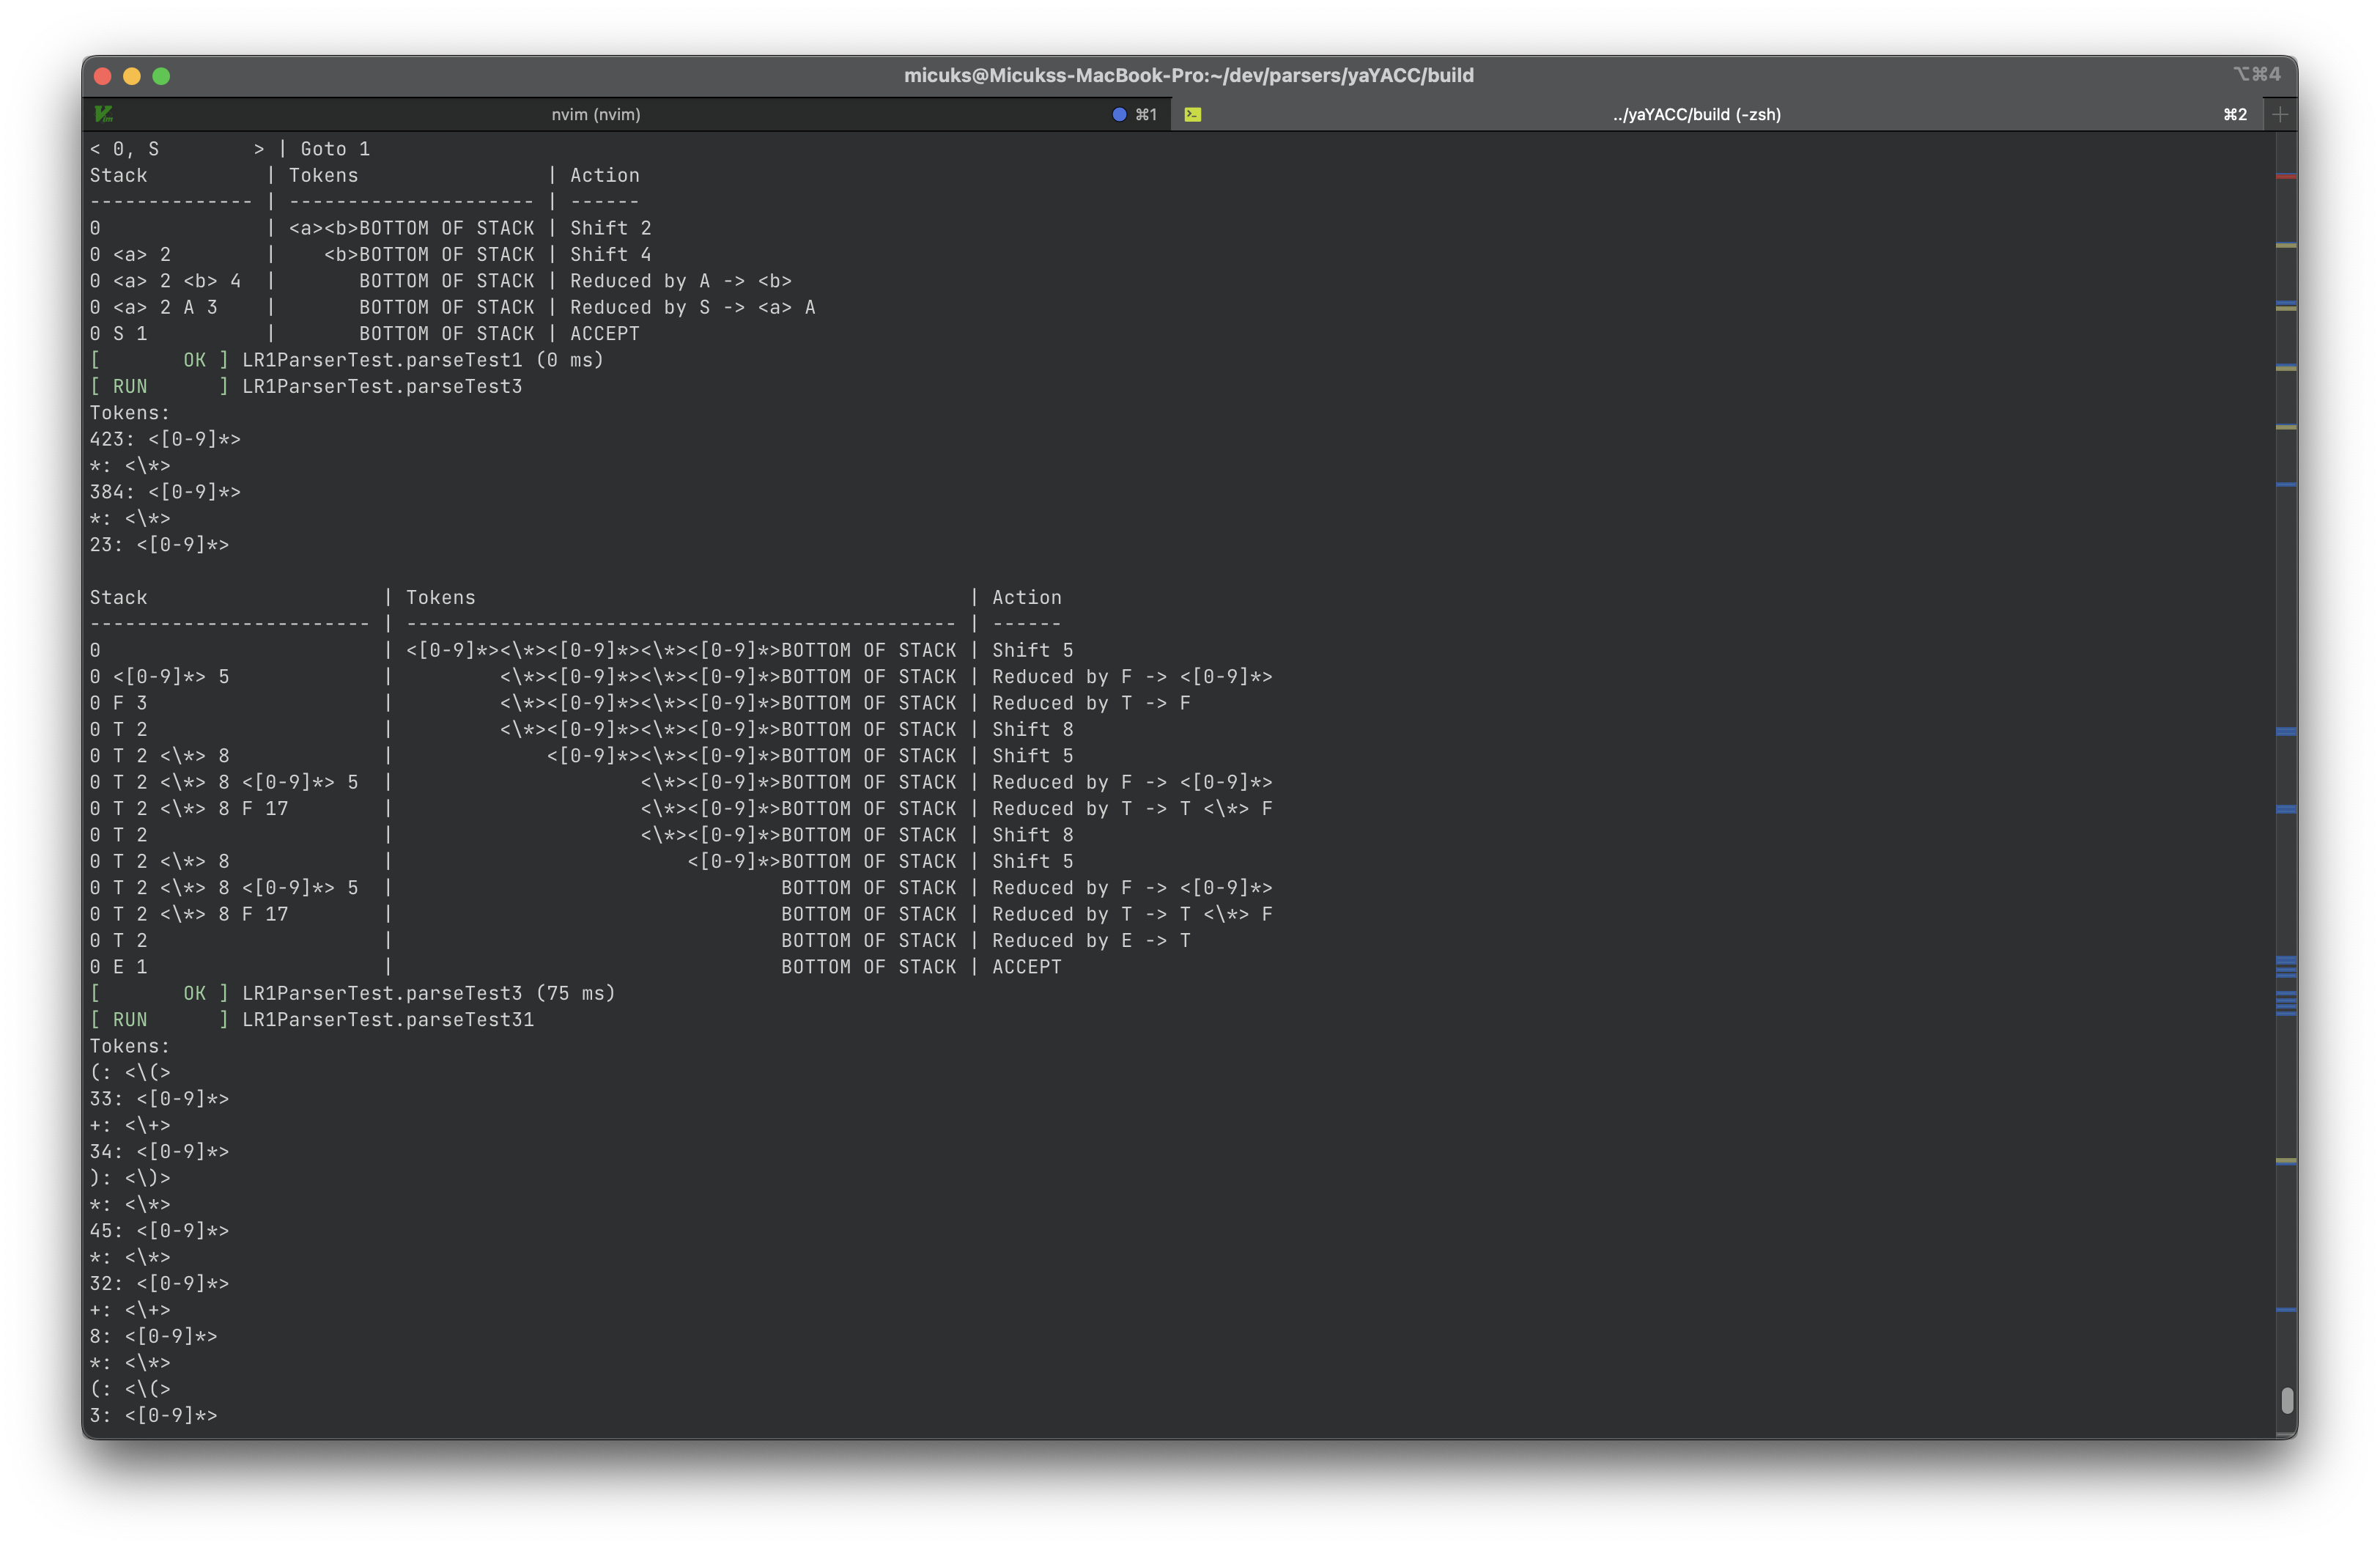
\includegraphics[width=0.95\textwidth]{figures/lr1复杂分析1.png}
	\end{center}
	\caption{复杂文法的LR1分析1}
	\label{fig:复杂文法的LR1分析1}
\end{figure}

\begin{figure}[ht!]
	\begin{center}
		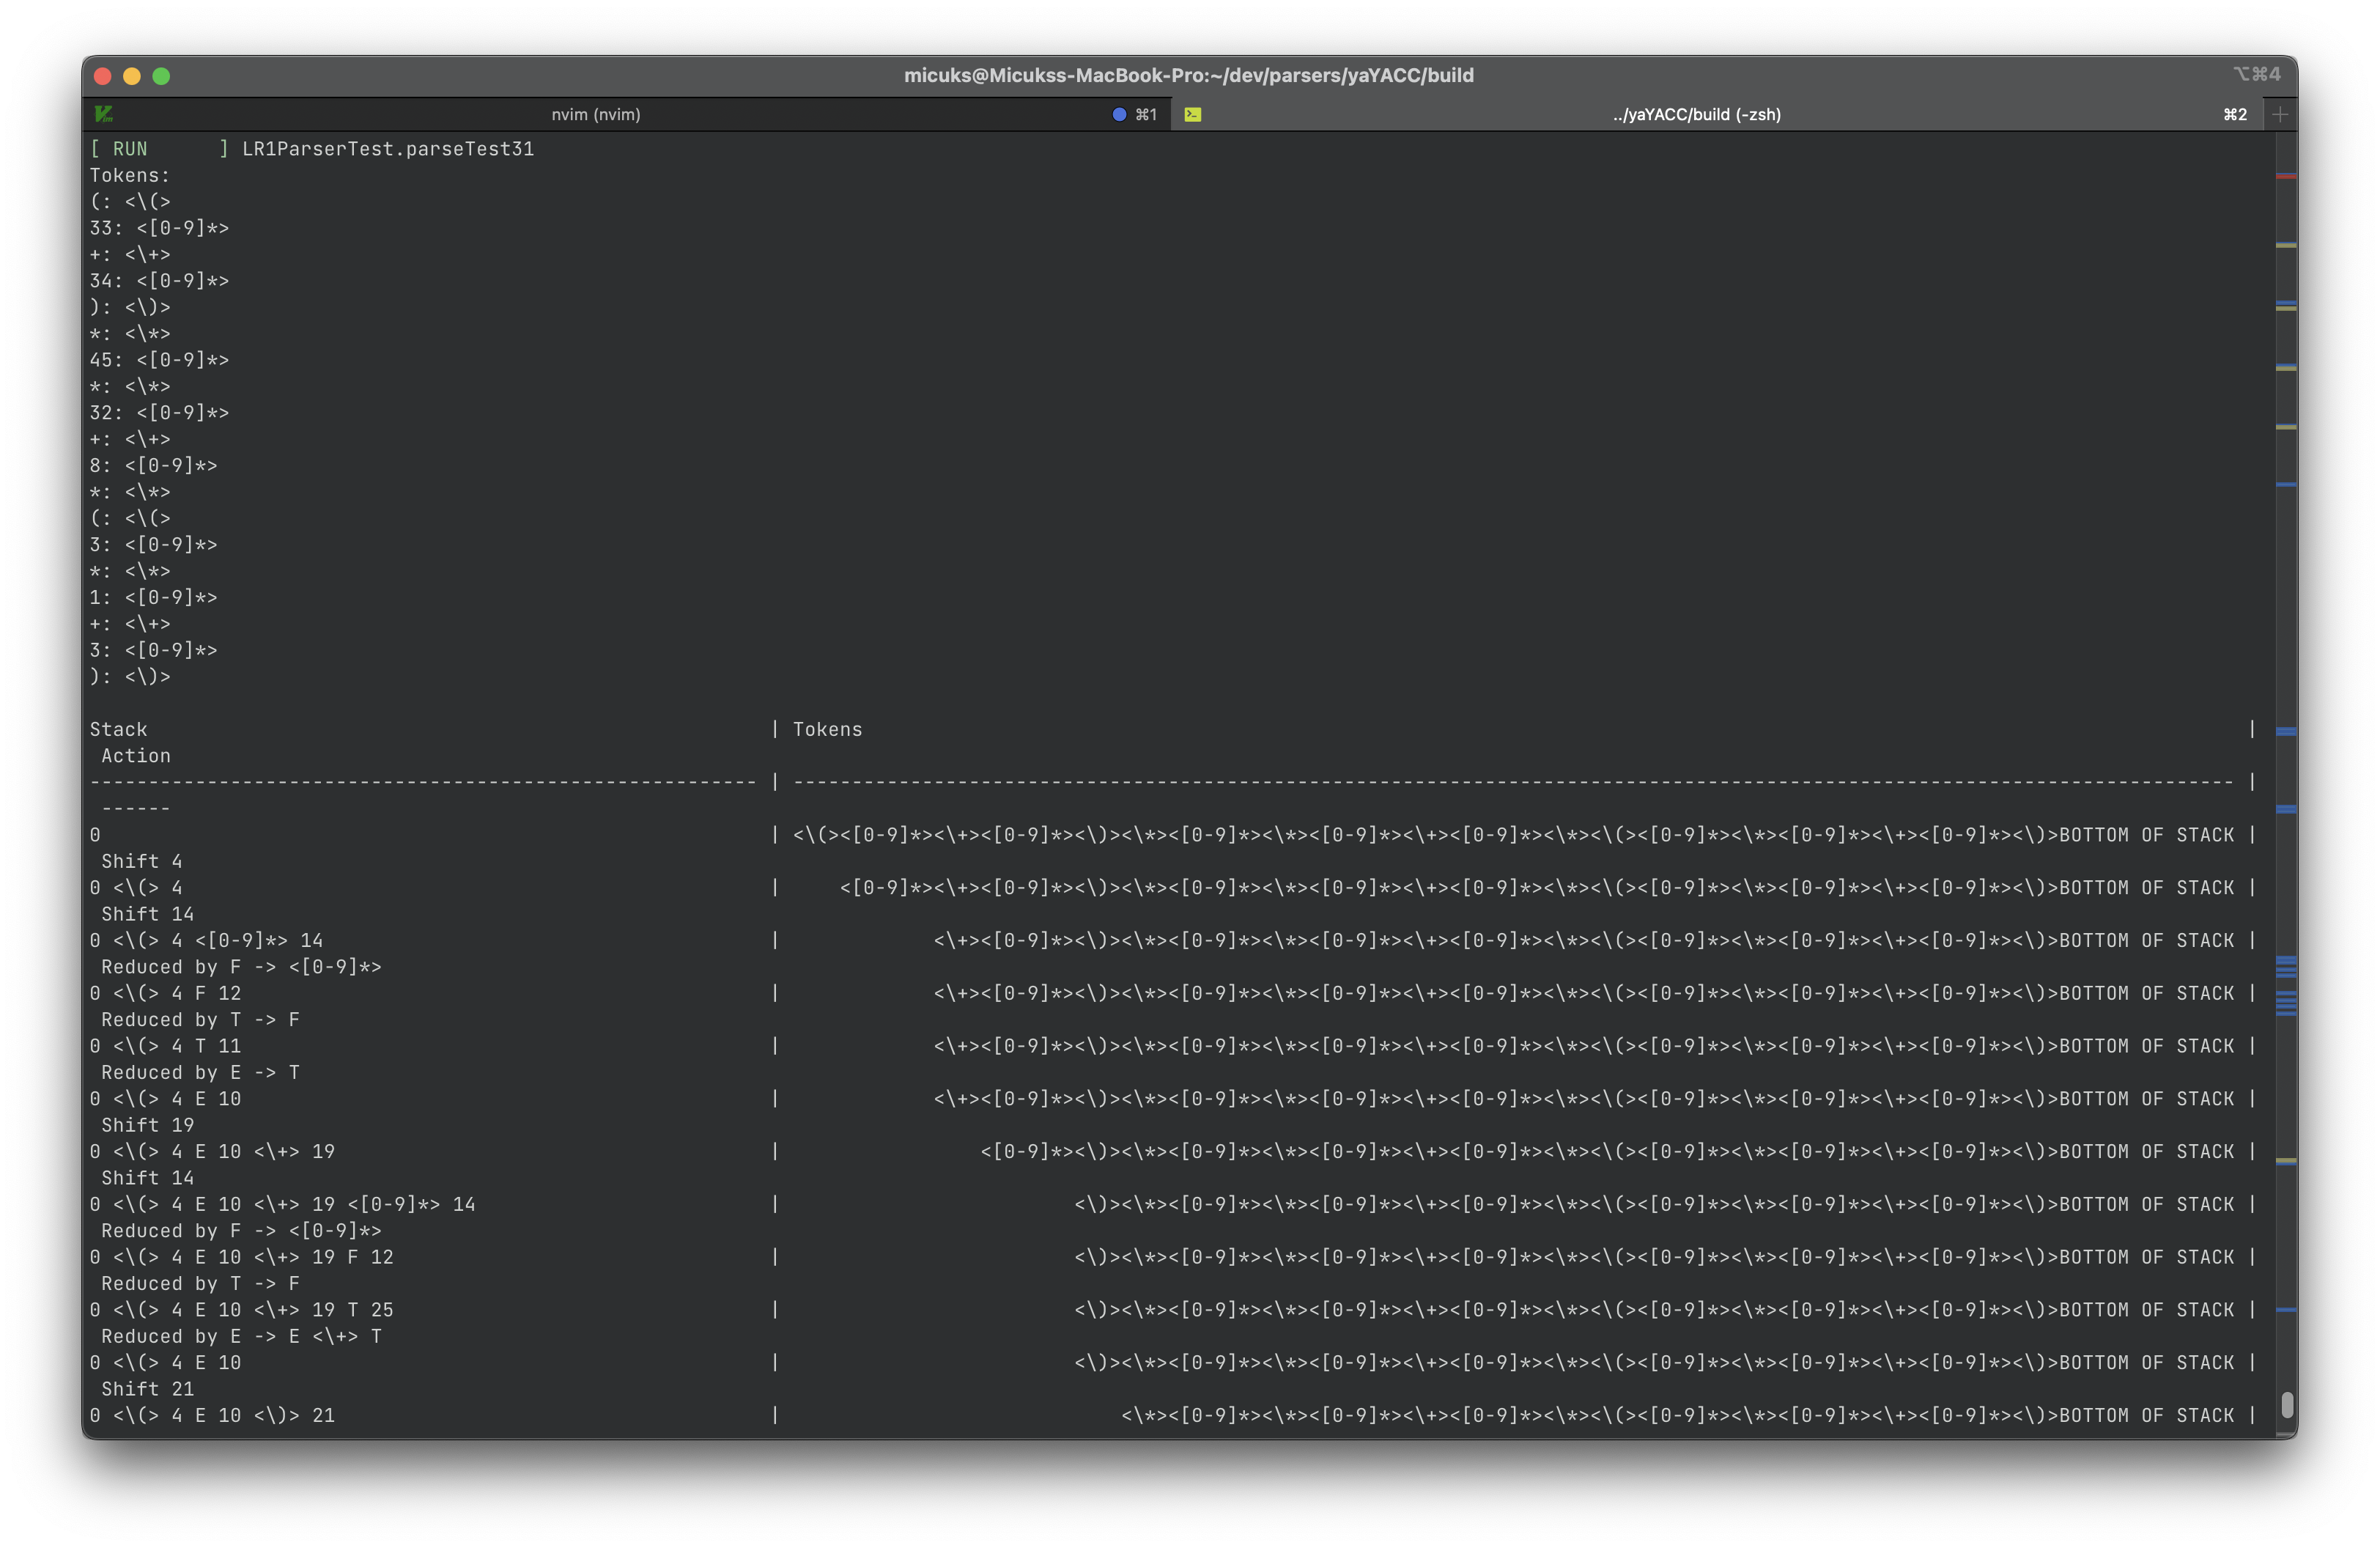
\includegraphics[width=0.95\textwidth]{figures/lr1复杂分析2.png}
	\end{center}
	\caption{复杂文法的LR1分析2}
	\label{fig:复杂文法的LR1分析2}
\end{figure}

对较复杂的输入串"(33+34)*(45*32)+8*(3*1+3)"进行分析, 结果为接受,
如图\ref{fig:复杂文法的LR1分析2}.
由于输入的文法中对数字均使用了相同的正则表达式表示, 所以Tokens看起来不清晰.
可以通过替换grammar文法文件解决, 例如将g3.txt中的<[0-9]*>替换为<0> | <1> | <2> |
... | <9>.

\begin{figure}[ht!]
	\begin{center}
		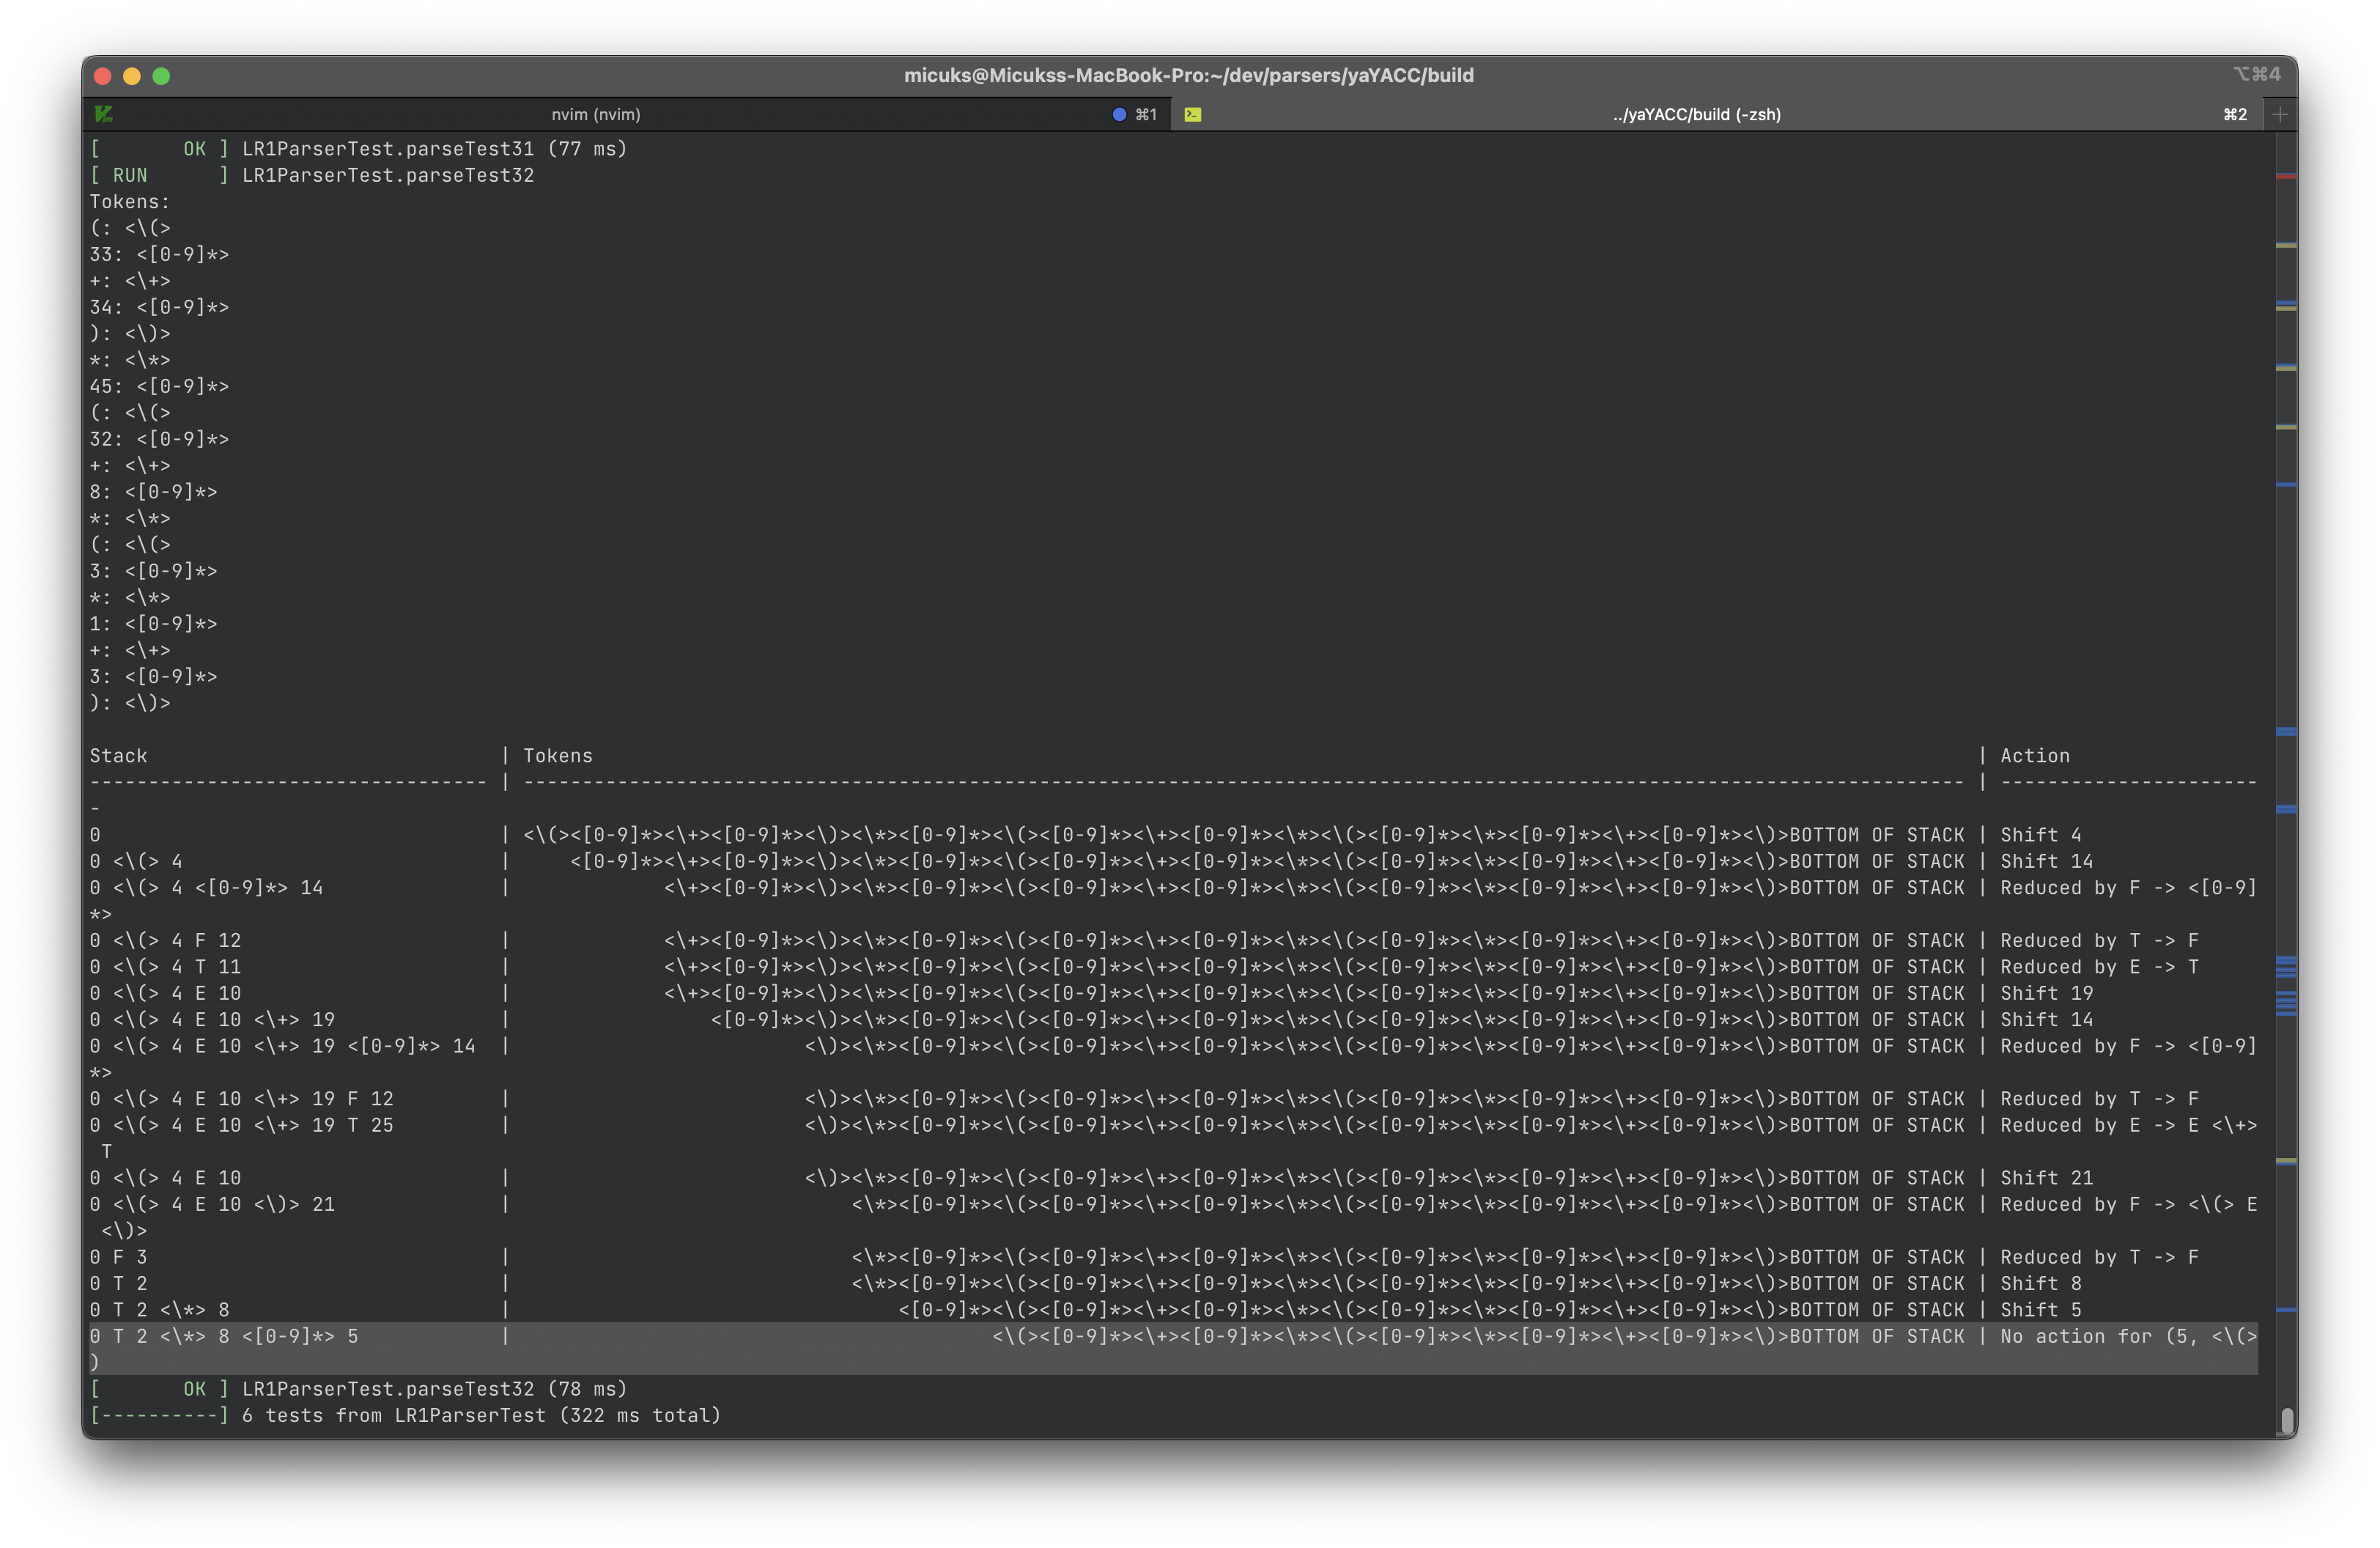
\includegraphics[width=0.95\textwidth]{figures/lr1复杂分析3.png}
	\end{center}
	\caption{复杂文法的LR1分析3}
	\label{fig:复杂文法的LR1分析3}
\end{figure}

对错误的输入能够正确拒绝, 如图\ref{fig:复杂文法的LR1分析3}.

\subsection{递归下降分析}
对较简单的输入串"423*384*23",
以及较复杂的输入串"(33+34)*(45*32)+8*(3*1+3)"进行测试, 得到输出均正确.

\begin{figure}[ht!]
	\begin{center}
		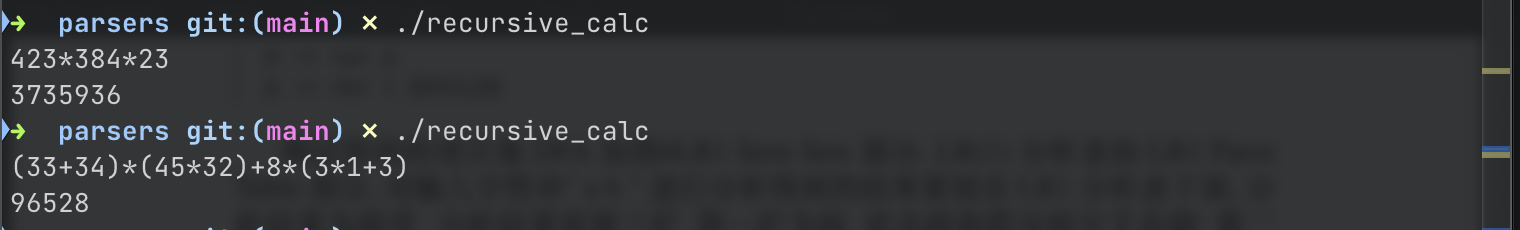
\includegraphics[width=0.95\textwidth]{figures/recursive_analysis.png}
	\end{center}
	\caption{递归下降分析测试}
	\label{fig:递归下降分析测试}
\end{figure}

\subsection{YACC生成的语法分析程序}

对较简单的输入串"423*384*23",
以及较复杂的输入串"(33+34)*(45*32)+8*(3*1+3)"进行测试, 得到输出均正确.
对于错误的输入串, 可以正确拒绝如图.

\begin{figure}[ht!]
	\begin{center}
		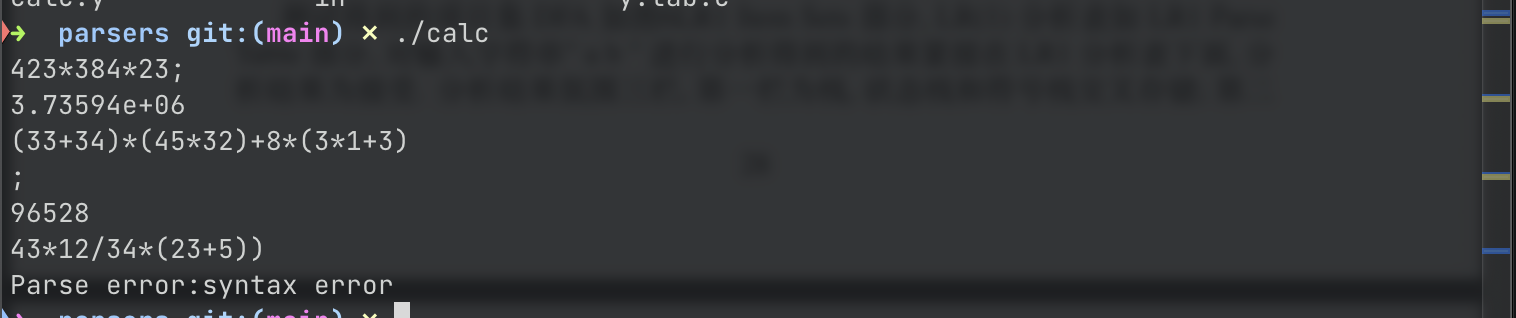
\includegraphics[width=0.95\textwidth]{figures/yacc_analysis.png}
	\end{center}
	\caption{YACC生成的语法分析程序测试}
	\label{fig:YACC生成的语法分析程序测试}
\end{figure}
